\documentclass[12pt,oneside]{mitthesis}
\usepackage{graphicx}
\usepackage{float}
\usepackage{textcomp}
\usepackage{caption}
\usepackage{subcaption}
\usepackage{siunitx}
% \usepackage{physics}
\usepackage{amssymb}
\usepackage{chemformula}
\usepackage{multirow}
\usepackage{makecell}
\usepackage{lgrind}
\usepackage{cmap}
\usepackage[T1]{fontenc}
\usepackage{indentfirst}
\usepackage{mathtools}
\usepackage{feynmp-auto}
\usepackage{svg}
\usepackage[greek,english]{babel}

\newcommand\omicron{o}

\usepackage[colorlinks=true,bookmarks=true,backref=page]{hyperref}
\usepackage{bookmark}
\hypersetup{
    breaklinks=true,
    allcolors=blue,
    linktoc=all
}

\usepackage{geometry}
\geometry{
    a4paper,
    left=1.5in,
    right=1.0in,
    top=1.0in,
    bottom=1.0in
}

\usepackage{footnote}
\makesavenoteenv{tabular}
\makesavenoteenv{table}

\usepackage{fancyhdr}
\fancypagestyle{plain}{
    \fancyhf{} % clear all header and footer fields
    \fancyhead[R]{\thepage} % page number in top right
    \renewcommand{\headrulewidth}{0pt}
    \renewcommand{\footrulewidth}{0pt}
}

\usepackage{lipsum}

\newcommand{\mysignrule}[0]{
    \rule{\linewidth}{0.5pt}\newline
}

\renewcommand\cellalign{tl}
\renewcommand\theadalign{tr}

\DeclareSIUnit\atm{atm}

% abs and norm definitions
\DeclarePairedDelimiter\abs{\lvert}{\rvert}%
\DeclarePairedDelimiter\norm{\lVert}{\rVert}%
% Swap the definition of \abs* and \norm*, so that \abs and \norm resizes the size of the brackets, and the starred version does not.
\makeatletter
\let\oldabs\abs
\def\abs{\@ifstar{\oldabs}{\oldabs*}}
\let\oldnorm\norm
\def\norm{\@ifstar{\oldnorm}{\oldnorm*}}
\makeatother

% bra ket notation
\newcommand{\bra}[1]{\langle#1\rvert} % Bra
\newcommand{\ket}[1]{\lvert#1\rangle} % Ket
\newcommand{\qprod}[2]{\langle#1|#2\rangle} %Inner Product
\newcommand{\braopket}[3]{\langle#1|#2|#3\rangle} % Matrix Element
\newcommand{\expect}[1]{\langle#1\rangle} % Expectation value

\usepackage{booktabs}

%-------------------------------------------
\begin{document}

\hypersetup{pageanchor=false}
\pagenumbering{roman}
\title{Ruling Out the Onset of Color Transparency up to $Q^2=\SI{14.2}{\giga\electronvolt\squared}$ in Quasielastic ${}^{12}C(e,e'p)$ Scattering}
\makeatletter
\bookmark[named=FirstPage]{\@title}
\makeatother

\makeatletter
\author{John Matter} \let\Author\@author
\newcommand{\hometown}{Moreno Valley, CA}

\prevdegrees{B.S., University of Califoria, Davis, 2012}
\department{Department of Physics}
\degree{Doctor of Philosophy}
\degreemonth{August}
\degreeyear{2021} \let\Year\@degreeyear
\thesisdate{August 13, 2021}
\makeatother

\supervisor{Nilanga Liyanage}{Professor}
\chairman{Kent Paschke}{Professor}

\makeatletter
\def\maketitle{\begin{titlepage}
\doublespacing
\vspace{0.0in}
\large
{\LARGE\bf \@title \par}
\@author \\
\hometown
\par
\@prevdegrees
\par
A Dissertation Presented to the Graduate Faculty \\
of the University of Virginia in Candidacy for the Degree of \\
\@degree
\par
\@department \\
University of Virginia \\
\@degreemonth, \@degreeyear \\
\vspace{1.0in}

\begin{flushright}
\begin{minipage}{0.45\linewidth}
\mysignrule{}
\mysignrule{}
\mysignrule{}
\mysignrule{}
\end{minipage}
\end{flushright}

\end{titlepage}}
\makeatother
\maketitle

% % Copyright page
% \pagenumbering{roman}
% \pagestyle{plain}
% \newpage
% \vspace*{\fill}
% \noindent \textcopyright Copyright by \Author {} \Year \\
% All Rights Reserved

\cleardoublepage

% Abstract page
\vspace{0.8in}
\pdfbookmark[0]{Abstract}{Abstract}
\section*{\center Abstract}
\noindent
Color Transparency (CT) is a prediction of QCD that at high momentum transfer
$Q ^2$, a system of quarks which would normally interact strongly with nuclear
matter could form a small color-neutral object whose compact transverse size
would be maintained for some distance, passing through the nucleus undisturbed.
A clear signature of CT would be a dramatic rise in nuclear transparency $T$
with increasing $Q^2$.
CT emerges as a deviation from Glauber multiple scattering
theory, which predicts constant $T$.
While a rise in nuclear transparency would provide an unequivocal validation of
QCD factorization theorems, the complex nature of nuclear
interactions renders its observation difficult to predict.
The E12-06-107 experiment at JLab measured $T$ in quasielastic electron-proton
scattering with carbon-12 and liquid hydrogen targets, for $Q^2$ between 8.0
and \SI{14.2}{\giga\electronvolt\squared}, a range over which models of CT
predicted that $T$ might differ appreciably from Glauber calculations.
Supported in part by US DOE grant DE-FG02-03ER41240.


\cleardoublepage

% Dedication page
\pdfbookmark[0]{Dedication}{Dedication}
\section*{Dedication}
\vspace{4cm}
\begin{center}
For Mormor \\
Josephine Anne Binnquist \\
14 Feb 1917 -- 3 Oct 2006
\end{center}

\begin{figure}[!h]
    \centering
    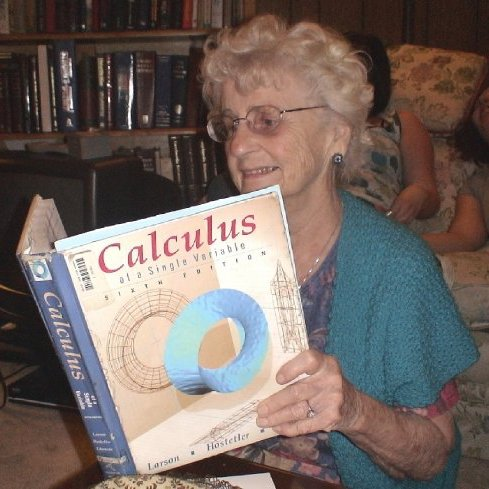
\includegraphics[width=0.6\textwidth]{mormor.jpg}
\end{figure}


\cleardoublepage
% Acknowledgemnt page
\pdfbookmark[0]{Acknowledgments}{Acknowledgments}
\section*{Acknowledgments}
First, I would like to thank my advisor, Nilanga Liyanage, for his guidance,
support, and enthusiasm.
I wouldn't be here without his tireless work finding research and funding
opportunities for me and his other students.

I would like to thank the members of my defense committee:
Phil Arras,
Simonetta Liuti,
and
Kent Paschke.

I would like to thank my collaborators on this experiment:
Dipangkar Dutta,
Holly Szumila-Vance,
Carlos Ayerbe Gayoso,
Latif Kabir,
and
Deepak Bhetuwal.

I would like to thank Krishni Wijesooriya, who I have worked with on and off
over the past several years.
I'm inspired by her drive to find new uses for existing information,
whether clinical CT scans or stray nuclear resonance fluorescence photons.

I would like to thank my parents and siblings for their love and
support over the years.

Thank you to Kathleen Larsen, for her love and patience.

Thank you to my dear friends:
Hicham Benhallam,
Jacob Boyd,
Kim McMasters,
Adam Smith,
and
Anney Traymany.

I would also like to thank the following people for
their contributions to my research and education:

Eric Aliotta,
Xinzhan Bai,
Hem Bhatt,
Deb Biswas,
Max Bychkov,
JP Chen,
Eric Christy,
Peter Cline,
Silviu Covrig,
Brad Cox,
Donal Day,
Danning Di,
Craig Dukes,
Burcu Duran,
Rolf Ent,
Debbie Eyer,
Howard Fenker,
Michael Fowler,
Dave Gaskell,
Kondo Gnanvo,
Craig Group,
Thir Gautam,
Beth Guyton,
Ole Hansen,
Tanja Horn,
Garth Huber,
Sarah Jarrett,
Siyu Jian,
Mark Jones,
Abishek Karki,
Joe Kiskis,
Israel Klich,
Eugene Kolomeisky,
Cynthia Keppel,
Chuck Long,
Dave Mack,
Simona Malace,
Rick Marshall,
Beverly Martyn,
Dave Meekins,
Hamlet Mkrtchyan,
Vladimir Nelyubin,
Huong Nguyen,
Brian Peter,
Eric Pooser,
Anuruddha Rathnayake,
James Rocillo,
Cass Sackett,
Faye Safley,
Brad Sawatzky,
Dawn Shifflett,
Tammie Shifflett,
Greg Smith,
the Spiliotis family,
Larry St. John,
Hank Thacker,
Al Tobias,
Diana Vaman,
April Wilson,
Bogdan Wojtsekhowski,
Steve Wood,
Bryan Wright,
Carlos Yero,
Jixie Zhang,
Xiaochao Zheng,
Rena Zieve,
and many more I'm sure I’ve forgotten.


\hypersetup{pageanchor=true}

\pagestyle{plain}
\include{contents}

\pagenumbering{arabic}
\chapter{Introduction}
\section{Atoms, Nuclei, and Nucleons}

Both the notion of the atom and the English word \textit{atom}
(from the Greek \textgreek{ἄτομος}---átomos---``uncuttable,''
itself composed of the etymological ``atoms''
\textgreek{ἀ}---a---``not''
and
\textgreek{τέμνω}---témnō---``I cut'') can be traced to the Presocratic Greek
philosophers Leucippus and Democritus~\cite{sep-atomism-ancient}.
They posited that the natural world consists of two fundamental
constituents---atoms and the void through which they move.


This theory was developed in response to the paradoxes of Zeno of
Elea, which appear to draw contradictory conclusions about ``plurality'' and
the possibility of motion, particularly if matter consists of infinitely divisible
constituent parts~\cite{sep-paradox-zeno}.
Zeno argued that traversing a finite distance required first traversing
infinitely many subdivisions of that distance---an apparent contradiction.
Democritus's model supposes the existence of a smallest subdivision, rendering
the finite distance to be traversed a sum of finitely many parts.
Various configurations of varying kinds, shapes, and sizes of Democritus's
atoms were thought to be the origins of the sensible properties of macroscopic
matter.
According to Democritus, these combinations of atoms collide with an animal's
sensory organs, giving rise to sensory experience.


In the early 19th century, John Dalton formulated the first modern concept of
the atom as the fundamental building block of chemical compounds.
His theory held that every chemical element is composed of atoms of identical
type and that different elements are composed of atoms of different size and
weight.
Chemical compounds are composed of whole numbers of atoms and reactions
involving different compounds consist of a rearrangement of the constituent
atoms.


In 1828, while studying the plant \textit{Clarkia pulchella} immersed in water
under a microscope,
botanist Robert Brown noted the irregular motion of the plant's pollen on the
surface of the water~\cite{Brown_1828}.
In 1905, Albert Einstein developed a model of this motion as arising from
collisions between the pollen and individual water molecules~\cite{Einstein_1905}.
% if I include this do I have to start talking about the history of molecular theory? seems tedious
French physicist Jean Perrin's measurements of the sedimentation of small
particles in liquid confirmed Einstein's hypothesis, work for which he was
awarded the Nobel Prize in 1926~\cite{Perrin_Nobel}.


Ernest Rutherford, Hans Geiger, and Ernest Marsden carried out a series of
experiments between 1908 and 1913 in which they fired a beam of alpha particles
at thin metal foils to study atomic-scale structure~\cite{Rutherford_1911}.
The distribution of scattered particles they observed suggested that the atom
is composed of a small, dense, positively charged nucleus surrounded by a cloud
of electrons.

In the century since, physicists have used other particle beams to study the
substructures of nuclei as well as the nucleons (i.e. protons and neutrons)
that compose nuclei.
The culmination of decades of such experiments is a theory called quantum
chromodynamics (QCD)---the theory that quarks and gluons are the fundamental
building blocks that make up hadrons, a category of composite particles that
includes protons and neutrons.
QCD also describes the interactions between such particles---the
\textit{strong nuclear force}.


QCD is part of the ``Standard Model'' of particle physics, which holds that
everything in the universe is made up of a handful of basic building blocks
whose interactions are governed by a few fundamental forces.
These building blocks, collectively called fermions, belong to two groups of
particles---quarks and leptons.
The quarks are typically found confined inside hadrons, while leptons can move
about more freely.
The interactions between these particles are mediated by force-carrying
particles called bosons that carry discrete packages of energy and momentum
between fermions.

Each of the three fundamental forces has one or more bosons associated with it.
The strong nuclear force, as mentioned above, has the gluon.
The electromagnetic force (quantum electrodynamics or QED) has the photon.
The weak nuclear force, responsible for beta decay among other things, has the
positively and negatively charged $W$ bosons and the neutral $Z$ boson.
There are a number of theories that have tried to incorporate the fourth
fundamental force, gravity, in a way that is consistent with the Standard
Model.
Unfortunately, this pursuit has proven difficult and no such theory has been
proven correct.
Fig~\ref{fig:Standard_Model_of_Elementary_Particles} displays the full list
of fundamental particles in the Standard Model, along with some of their
properties.

\begin{figure}[!h]
    \centering
    \includegraphics[width=0.6\textwidth]{chap1/Standard_Model_of_Elementary_Particles.pdf}
    \caption{The elementary particles of the Standard Model. Reproduced from
             Wikimedia~\cite{standard_model_wikimedia}.
            }
    \label{fig:Standard_Model_of_Elementary_Particles}
\end{figure}


\section{Electron scattering}
The Thomas Jefferson National Accelerator Facility (JLab) in Newport News, VA
is home to the Continuous Electron Beam Accelerator Facility (CEBAF).
The CEBAF beam delivers a beam of high energy polarized electrons to four
experimental halls.
Most JLab experiments study the debris produced when the electron beam
hits a fixed nuclear target.
By studying this debris, physicists are able to obtain new insights into
nuclear and nucleon structure, exotic configurations of quarks, and other
features of QCD.
Electron beams such as the CEBAF are powerful tools for studying nuclear
structure
because the processes involved in electron-nucleus scattering experiments are
governed by QED (a theory which is very well understood and calculable to high
degrees of precision).

\begin{figure}[H]
    \centering
    \vspace{1cm}
        \begin{fmffile}{chap1/elastic_scattering}
            \setlength{\unitlength}{1cm}
            \begin{fmfgraph*}(8,5)
                \fmfleft{ie,oe}
                \fmfright{ip,op}

                \fmflabel{$(E_e,\vec{p}_e)$}{ie}
                \fmflabel{$(E'_e,\vec{p'}_e)$}{oe}

                \fmflabel{$(E_p,\vec{p}_p)$}{ip}
                \fmflabel{$(E'_p,\vec{p'}_p)$}{op}

                \fmf{fermion}{ie,v1,oe}
                \fmf{photon,label=$q_\mu=(\nu,,\vec{q})$}{v1,v2}
                \fmf{fermion}{ip,v2,op}
            \end{fmfgraph*}
        \end{fmffile}
    \vspace{1cm}
    \caption{Feynman diagram for elastic $ep$ scattering.}
    \label{fig:feynman_ep}
\end{figure}

Consider a situation in which an electron and proton collide.
The tree-level diagram for this process is shown in Fig~\ref{fig:feynman_ep}.
Let $p_e^\mu=(E_e,\vec{p}_e)$ be the incoming four-momentum of the electron and
${p'}_e^\mu=(E'_e,\vec{p'}_e)$ be its outgoing four-momentum.
Similarly, let $p_p^\mu$ and ${p'}_p^\mu$ be the incoming and outgoing
four-momenta of the proton.
The virtual photon carries a four-momentum
$q^\mu=(\nu,\vec{q})=(E_e-E'_e,\vec{p}_e-\vec{p'}_e)$ between the two
particles.
An important quantity defined for such processes is the four-momentum transfer
squared $Q^2=-q^\mu q_\mu$.
Similarly, $\nu=E_e-E'_e$ is the energy transfer.

\textit{Elastic scattering} is a process in which an electron and proton
collide, and both particles retain their identities.
This process can be seen as a distinct peak at $Q^2=2m_p\nu$ on the bottom axis
labeled ``PROTON'' in Fig~\ref{fig:nuclear_response_function}.
This figure is a schematic representation of the nuclear response
function\footnote{The nuclear response function can be thought of as the
probability for an interaction to occur between an electron and a proton or
nucleus at a given value of $Q^2$ and $\nu$.} as a function of $Q^2$ and $\nu$.

For a fixed value of $Q^2$, higher energy transfers $\nu$ result in first
resonances of the proton and, as the virtual photon probes smaller and
smaller distances, eventually deep inelastic scattering (DIS).
DIS processes are possible because the proton is not a point-like particle
without a substructure, but rather a composite particle composed of quarks.
The DIS region extends to electron-nucleus scattering at larger $\nu$ (see the
middle axis labeled ``NUCLEUS.''
In DIS events, quarks can be knocked out of protons and neutrons to form other
hadrons such as pions and kaons.

At lower values of $\nu$ for fixed $Q^2$, there is a peak labeled
quasi-free scattering, which is another term for \textit{quasielastic
scattering}.
This is a process in which the struck proton retains its identity and holds
onto its constituent quarks.
The process ``looks'' more like elastic scattering involving a free proton than
it does an inelastic process.

\begin{figure}[!h]
    \centering
    \includegraphics[width=1.0\textwidth]{chap1/nuclear_response_function_new.pdf}
    \caption[Schematic representation of the nuclear response function.]{
             A schematic representation of the nuclear response function,
             illustrating the phenomena probed by electron-nucleus scatterying
             in different regions of energy and momentum transfer.
             Reproduced from Ref~\cite{Frois_1985}.
            }
    \label{fig:nuclear_response_function}
\end{figure}

Quasielastic scattering is one type of scattering process that can be studied
in detail at JLab in Hall C using a pair of apparatuses called spectrometers.
If both spectrometers are used in tandem to collect both the scattered electron
and ejected proton, this is called \textit{exclusive} quasielastic scattering.
Inclusive scattering detects only one of the particles, leaving some abmiguity
about exactly what process led to its being scattered into a spectrometer.


Because the ejected proton interacts with the residual nucleons via the strong
force, it will interact with the nuclear medium as it exits the nucleus.
This ``rescattering'' process is well-described by Glauber multiple scattering
theory~\cite{Glauber_1959}.
However, there is a distinctive prediction~\cite{Mueller_1982,Brodsky_1982}
arising from QCD that in exclusive processes at large $Q^2$, initial and final
state interactions (ISI and FSI) such as Glauber multiple scattering vanish.
At sufficienctly large $Q^2$, a proton ejected from a nucleus in quasielastic
scattering behaves as if it were a free proton participating in elastic
scattering.

\section{Color Transparency}
Color transparency (CT), a characteristic prediction of QCD, refers to the
reduction of initial and final state interactions between a hadron and the
nuclear medium in exclusive processes at large momentum transfer $Q^2$.
The concept was first independently proposed by Mueller and Brodsky in the
context of perturbative QCD, but was later shown to arise in nonperturbative
models.
% An analogue of CT can be seen in QED--a small $e^+e^-$ pair has a small cross
% section determined by its dipole moment.


There are three requirements for the observation of CT in an experiment:
\begin{itemize}
    \item Squeezing: the formation of a small configuration of quarks, sometimes
          referred to as a point-like configuration (PLC)
    \item Interactions between the PLC and the nuclear medium are attenuated
          because of its small size
    \item Freezing: the PLC maintains its small size over a distance comparable
          to or greater than the nuclear radius
\end{itemize}

There is some evidence for the existence of and onset of CT in experiments
involving mesons.
The results of experiments involving baryons are a mixed bag; some results are
consistent with the absence of CT and others are ambiguous and cannot be
attributed to CT alone.
These experiments and relevant theoretical models and considerations are
discussed in Chapter 2.


In experiments studying the color transparency phenomenon, a common observable
is the nuclear transparency.
It is generally of the form $T=\sigma_A/A\sigma_0$,
the ratio of
the per-nucleon cross section for some exclusive scattering process
to
the cross section for the same process on a free nucleon.
Nuclear transparency can be thought of as the probability that a hadron
produced in a scattering process will exit the nucleus without rescattering
from another nucleon.


Previous experiments have used slightly different definitions of nuclear
transparency depending on the experiment's particulars.
Studies of $A(p,2p)$, quasielastic proton knockout using a proton beam,
at Brookhaven National Lab (BNL)~\cite{Carroll_1988, Mardor_1998, Leksanov_2001, Aclander_2004}
used the ratio of $\frac{d\sigma}{dt}$,
where $t$ is the four-momentum transfer squared.
Studies of $A(e,e'p)$, quasielastic electron scattering,
at MIT-Bates~\cite{Garino_1992},
SLAC~\cite{Makins_1994, ONeill_1995}
and Jefferson Lab (JLab)~\cite{Abbot_1998, Garrow_2002, Rohe_2005}
used the ratio of charge-normalized yields $Y$ measured in experiment
and from Monte Carlo simulation, $T=Y^{exp}/Y^{MC}$.
Studies of $A(e,e'\pi^+)$, pion electroproduction,
at JLab~\cite{Clasie_2007, Qian_2010}
used the super-ratio of the ratio of yields from experiment and simulation
for a nucleus with $A$ nucleons in the numerator and hydrogen in the
denominator,
$T= \big(Y^{exp}/Y^{MC}\big)_{A} / \big(Y^{exp}/Y^{MC}\big)_{H}$.


Traditional Glauber multiple scattering theory predicts that $T$ is constant as
$Q^2$ increases.
In this picture, the transparency should follow the same
energy dependence of the nucleon-nucleon scattering cross sections which,
as shown in Fig~\ref{fig:pdg_nucleon_nucleon_cross_section}.
are relatively constant between lab momenta of
\SI{1}{\giga\electronvolt} and \SI{1}{\tera\electronvolt}.
The reduction of initial/final state interactions predicted by CT results in an
increase in nuclear transparency with $Q^2$.
An illustration of this behavior is shown in Fig~\ref{fig:CT_toy_prediction}.

\begin{figure}[!h]
    \centering
    \begin{subfigure}[b]{1.0\textwidth}
        \centering
        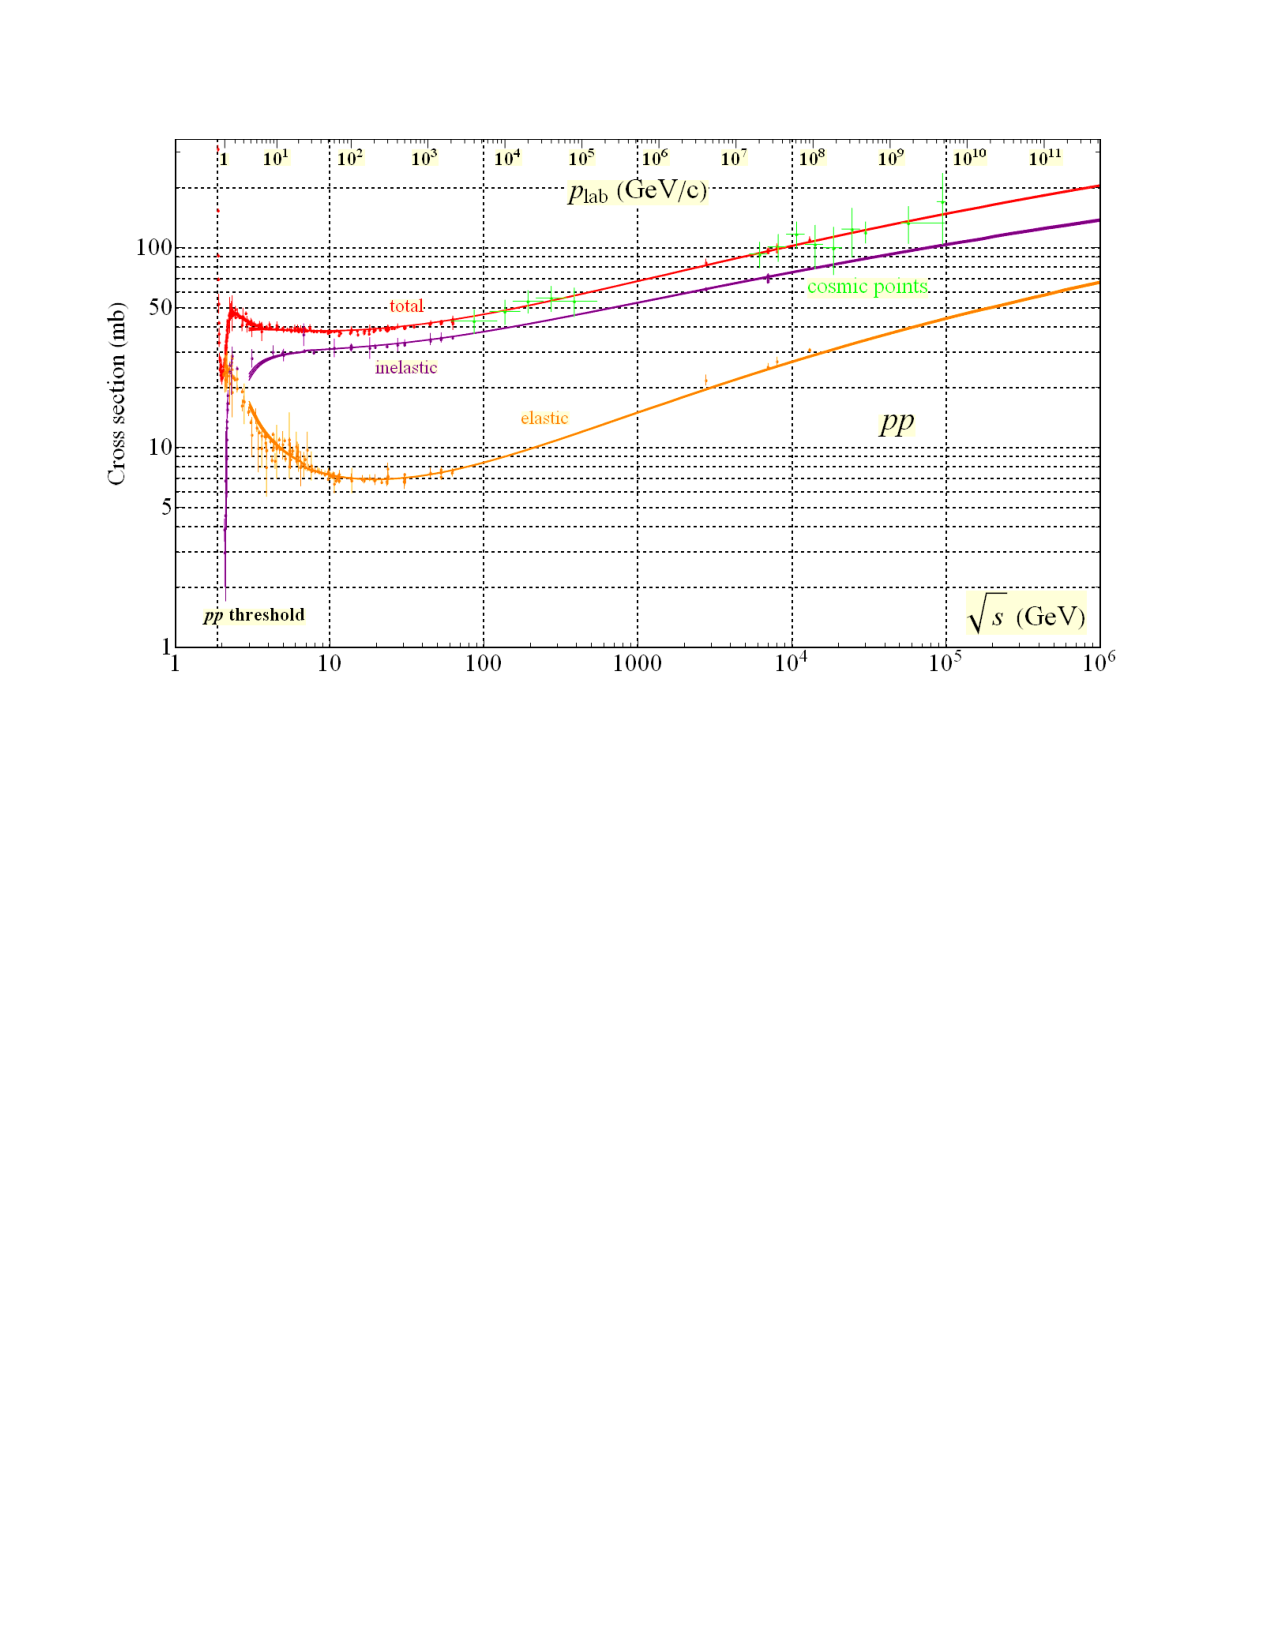
\includegraphics[width=1.0\textwidth]{chap2/pdg_pp_cross_section.pdf}
        \caption[Total, elastic, and inelastic $pp$ cross sections versus
                 $p_{lab}$ and $\sqrt{s}$.]{
                 Total, elastic, and inelastic $pp$ cross sections versus
                 $p_{lab}$ and $\sqrt{s}$.
                }
        \label{fig:pdg_pp_cross_section}
    \end{subfigure}
    \vspace{0.1cm}
    \\
    \begin{subfigure}[b]{1.0\textwidth}
        \centering
        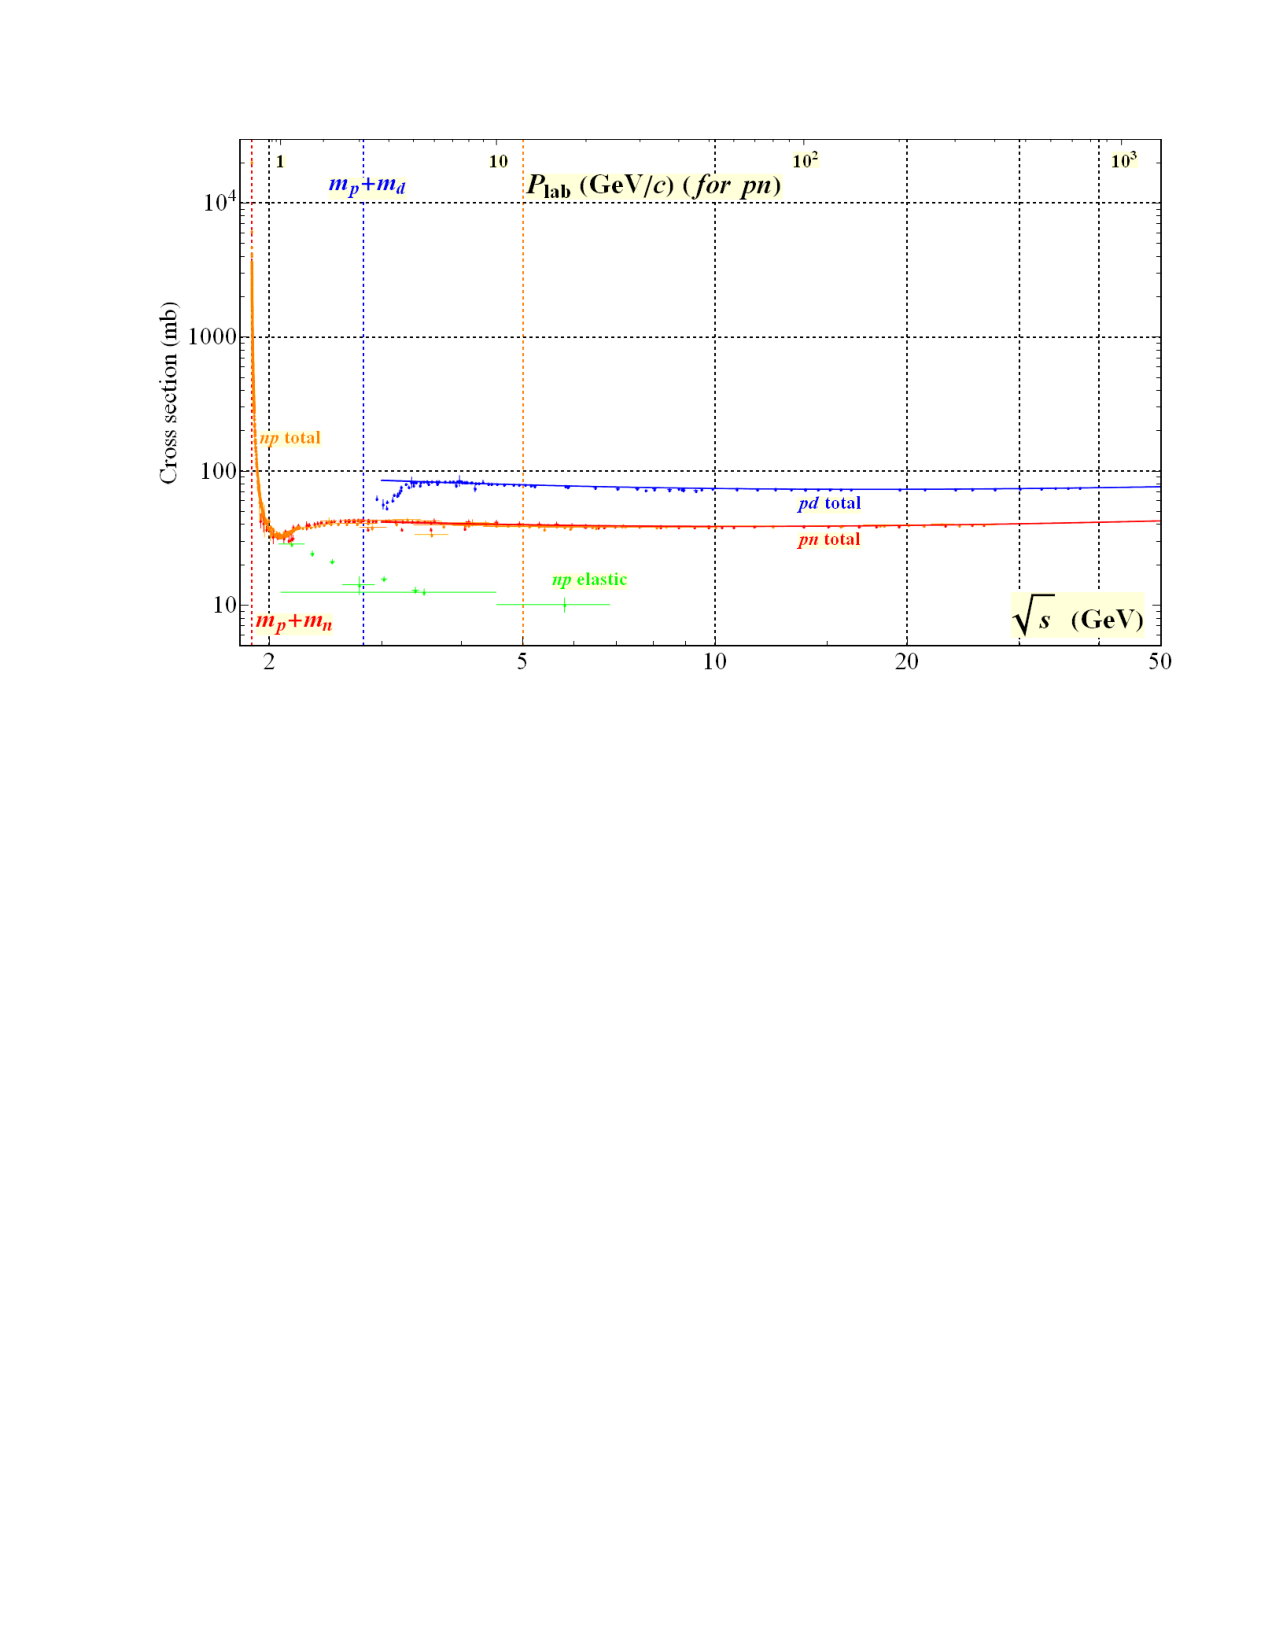
\includegraphics[width=1.0\textwidth]{chap2/pdg_pn_cross_section.pdf}
        \caption[Total $pn$ and $pd$ cross sections versus
                 $p_{lab}$ and $\sqrt{s}$.]{
                 Total $pn$ and $pd$ cross sections versus
                 $p_{lab}$ and $\sqrt{s}$.
                }
        \label{fig:pdg_pn_cross_section}
    \end{subfigure}
    \caption[Total, elastic, and inelastic $pp$, $pn$, and $pd$, cross sections
             versus lab momentum $p_{lab}$ and center of mass energy $\sqrt{s}$.]{
             Total, elastic, and inelastic $pp$, $pn$, and $pd$, cross sections
             versus lab momentum $p_{lab}$ and center of mass energy $\sqrt{s}$.
             Note that the total cross section is relatively constant over
             the range of momenta studied in E12-06-107, about
             \SIrange{4}{10}{\giga\electronvolt}.
             Figure reproduced from Ref~\cite{pdg_2020}.
             }
    \label{fig:pdg_nucleon_nucleon_cross_section}
\end{figure}


\begin{figure}[!h]
    \centering
    \includegraphics[width=0.8\textwidth]{chap1/CT_toy_prediction.pdf}
    \caption[ An illustration of the $Q^2$ dependence of nuclear transparency $T$
            for three scenarios.]{
            An illustration of the $Q^2$ dependence of nuclear transparency $T$
            for three scenarios.
            The blue line illustrates the prediction of the Glauber model,
            which has constant $T$ as $Q^2$ increases.
            The red line illustrates that for full color transparency, $T=1$;
            in this scenario there are no final state interactions between the
            ejected proton and the rest of the nucleus.
            The green line illustrates the scenario where the transparency
            begins to deviate from the Glauber prediction above an onset
            $Q_0^2$ and approach $T=1$ with increasing $Q^2$.
            }
    \label{fig:CT_toy_prediction}
\end{figure}

\section{Nuclear Transparency}
In order to quantify the effects of final state interactions in interactions
such as quasielastic scattering, experiments measure nuclear transparency--the
ratio of
the measured interaction cross section
to
the cross section calculated in the PWIA.
The definition of transparency used in this work is the same as that used by
previous experiments experiments looking for the onset of CT in
${}^{12}C(e,e'p)$,
\begin{equation} \label{eqn:transparency_definition}
    T(Q^2) = \frac{\int_{V} d^{3} p_{m} d E_{m} Y^{exp }(E_{m}, \vec{p}_{m})}
                  {\int_{V} d^{3} p_{m} d E_{m} Y^{PWIA}(E_{m}, \vec{p}_{m})}
\end{equation}
where $Y^{exp}$ and $Y^{PWIA}$ are charge-normalized yields from experiment and
simulation.

The experimental yield is given by $Y=N/Q$, where $N$ is the total number of
scattering events measured per integrated beam charge $Q$ incident on the
target.
If the beam current is $j$ and the target has density $\rho$ and length $l$,
then the total number of events is $N=\int_{t_1}^{t_2} j \rho l \sigma dt$,
integrated over the total time the beam was on $t_2-t_1$.
The simulated yield is generated by SIMC, a Monte Carlo simulation of the PWIA.
The details of the simulation are described in
Section~\ref{sec:simulation_intro} and Appendix~\ref{app:simc}.

The yields are integrated over a volume of missing energy and momentum phase
space $V$, defined by the cuts $E_m < \SI{80}{\mega\electronvolt}$ and
$|\vec{p}_m| < \SI{300}{\mega\electronvolt}$.
These cuts prevent inelastic contributions from pion production and ensure that
the recoil nucleus remains in its ground state.
Nuclear transparency can be thought of as the probability that a struck proton
will exit the nucleus without rescattering from another nucleon.

\input{chap1/pwia}
\section{Quasielastic Scattering and the Glauber Approximation}
Benhar et. al~\cite{Benhar_2000, Rohe_2005} present a calculation of nuclear
transparency for quasielastic scattering in the correlated Glauber
approximation.
What follows is a summary of their method.

Let
$\Psi_0^{(A)}$ be the ground state wave function of the $A$-body target nucleus,
$\Psi_{\vec{p}}$ the final state wave function of the ejected proton with momentum $\vec{p}$,
and
$\Psi_f^{(A-1)}$ is the final state wave function of the residual $(A-1)$ nucleus.
Then, in terms of
annihilation $\hat{a}_{\vec{k}}$ and
creation operators $\hat{a}_{\vec{k}}^\dagger$
for nucleon states of momentum $\vec{k}$,
the matrix amplitude for $A(e,e'p)$ scattering can be
written
\begin{equation}
    \mathcal{M} = \braopket{\Psi_{\vec{p}}^{(A-1)}}
                           {\sum_{\vec{k}} \hat{a}^\dagger_{\vec{k}+\vec{q}} \hat{a}_{\vec{k}}}
                           {\Psi_0^{(A)}}
\end{equation}


The Hamiltonian of the full $A$-body system can be rewritten to separate the
final state interactions between the ejected proton and the spectator nucleons
\begin{equation}
    \hat{H}_{A} = \hat{H}_0 + \hat{H}_{FSI} = (\hat{H}_{A-1} + T_1) + \hat{H}_{FSI}
\end{equation}
where $H_{A_1}$ is the Hamiltonian of the recoil nucleus
$T_1$ is the kinetic energy operator for the ejected proton
and
$\hat{H}_{FSI}$ contains the final state interactions.


Then, if the state $\Phi_{\vec{p}}$ is an eigenstate of $H_0$ that describes
the system in the absence of FSI, there is a scattering operator
$\Omega_{\vec{p}}$ such that
\begin{equation}
    \ket{\Psi_{\vec{p}}} = \Omega_{\vec{p}} \ket{\Phi_{\vec{p}}}
\end{equation}


Formally, this operator can be written
\begin{align}
    \Omega_{\vec{p}} &= \lim_{t\rightarrow\infty} e^{-i\hat{H}_At}e^{-i\hat{H}_0t} \\
                     &= \lim_{t\rightarrow\infty} \hat{T} e^{-\int_0^t dt' \hat{H}_{FSI}(t')}
\end{align}
where $\hat{T}$ is the time ordering operator and
\begin{equation}
    \hat{H}_{FSI}(t) = e^{i\hat{H}_0t} \hat{H}_{FSI} e^{-i\hat{H}_0t}
\end{equation}

Calculating this expression for a realistic Hamiltonian is difficult, but under
appropriate circumstances the Glauber approximation~\cite{Glauber_1959} can be
used to simplify this expression.
The Glauber approximation assumes that
the ejected proton moves in a straight line without rescattering
(the eikonal approximation)
and
the spectator nucleons can be treated as fixed
(the frozen approximation).

Assume the spectator nucleons are frozen at positions
$\vec{r}_j = z_j \hat{z} + \vec{b}_j$
where the $\hat{z}$ axis lies along the path of the ejected proton
and $\vec{b}_j$ are perpendicular to $\hat{z}$.

Let $R=\left\{ \vec{r}_1,\vec{r}_2,\ldots,\vec{r}_A \right\}$ be the
spatial configuration of the full $A$-body system.
In the correlated Glauber approximation, the scattering operator can be written
in coordinate space
\begin{align}
    \Omega_{\vec{p}}(R) \equiv \braopket{R}{\Omega_{\vec{p}}}{R}
        = \hat{P}_z \bigg[ 1 &- \sum_{j=2} \theta(z_j-z_1) \Gamma(\vec{b}_j-\vec{b}) \nonumber \\
                        &+ \sum_{j=2,k>j} \theta(z_j-z_1) \Gamma(\vec{b}_j-\vec{b}) \theta(z_k-z_1) \Gamma(\vec{b}_k) \nonumber \\
                        &- \cdots \bigg]
\end{align}
where $\hat{P}_z$ is a $z$-ordering operator preventing backscattering of the
ejected proton and the step functions $\theta(z)$ ensure causality.
The profile function $\Gamma(\vec{b})$ is a function of impact parameter
$\vec{b}$ and contains all the information about the scattering process.
It is a Fourier transform of the scattering amplitude $f(\vec{k}_t)$ which can
be extracted from measured cross sections.
\begin{equation}
    \Gamma(\vec{b}) = -\frac{i}{2}\int \frac{d^2k_t}{(2\pi)^2} e^{-\vec{k}_t \cdot \vec{b}} f(\vec{k}_t)
\end{equation}

The scattering amplitude takes the parameterized form
\begin{equation}
    f(\vec{k}_t) = i \sigma_{tot} (1-i\epsilon) e^{-k_t^2/2B}
\end{equation}
where $\epsilon$ is the ratio of the scattering amplitude's real and imaginary
parts and
$B$ is a slope parameter.

Let $\rho_p(\vec{r})$ be the proton density in a target nucleus with $Z$
protons.
Then the transparency is
\begin{equation}
    T = \frac{1}{Z} \int d^3r \rho(\vec{r}) \left| \Omega_{\vec{p}}(\vec{r})\right|^2
\end{equation}

The integrand can be expanded in terms of $n$-body distribution functions
$\rho^{(n)}_{p N \ldots N}(\vec{r}_1, \vec{r}_2, \cdots, \vec{r}_n)$ that express the
joint probability of finding the ejected proton at $\vec{r}_1$ and the $n-1$
spectator nucleons at positions $\{\vec{r}_2, \cdots, \vec{r}_n\}$.

\begin{align}
    \rho_{p}(\vec{r}_1)&\left| \Omega_{\vec{p}}(\vec{r})\right|^2 = \nonumber \\
        &1 - \frac{1}{\rho_{p}(\vec{r}_1)} \bigg[ \int d^3 \vec{r}_2 \theta(z_2-z)\Gamma(\vec{b}_2-\vec{b}) \rho^{(2)}_{pN}(\vec{r}_1,\vec{r}_2) \nonumber \\
            - &\int d^3 \vec{r}_2 d^3 \vec{r}_3 \theta(z_2-z)\Gamma(\vec{b}_2-\vec{b}) \theta(z_3-z)\Gamma(\vec{b}_3-\vec{b}) \rho^{(3)}_{pNN}(\vec{r}_1,\vec{r}_2, \vec{r}_3) \nonumber \\
            + &\int d^3 \vec{r}_2 d^3 \vec{r}_3 d^3 \vec{r}_4 \cdots \bigg]
\end{align}

The quantity in brackets contains the effects of final state interactions,
which result in a decrease in transparency from the PWIA result, $T=1$.
Each term represents a contributions from $n-1$ rescatterings.
The single rescattering term can be written as
$\rho^{(2)}_{pN}(\vec{r}_1,\vec{r}_2)=\rho_p(\vec{r}_1)\rho_N(\vec{r}_2)g(\vec{r}_1,\vec{r}_2)$,
where the function $g(\vec{r}_1,\vec{r}_2)$ describes the correlations between
nucleons~\cite{Schiavilla_1987}.
At short ranges $r=\norm{\vec{r}_1-\vec{r}_2}$, $g(r)\ll1$ because of the
strongly repulsive core of the nucleon-nucleon interaction.
At large $r$, $g(r) \rightarrow 1$ because of asymptotic freedom.

\subsection{Pandharipande et al.}
%The Glauber approximation~\cite{Glauber_1959} supposes that a struck proton
%with momentum $k$ and energy $E$, after quasielastic scattering, subsequently
%scatters from spectator nucleons at angles $\theta$ primarily in the
%forward direction.
%More precisely, if $a$ and $V$ are the radius and strength of the
%nucleon-nucleon interaction, this requires
%$V/E \ll 1$,
%$ka \gg 1$,
%and
%$\theta^2 k a \ll 1$.
%The wavefunction of the proton in these conditions can be written as
%%TODO: clean this up a little and clarify some variables; I'm trying to draw a link between a general Glauber summary and the specifics of the Pandharipande/Pieper paper
%\begin{equation} \label{eqn:eikonal_approximation}
%    \psi(\vec{r}) = e^{i\vec{k}\cdot\vec{r}}
%            \exp{ -\frac{1}{2} \int_{z'}^{z} dz'' \sigma(z'') \rho(\vec{r''}) }
%\end{equation}


This experiment takes the work of Pandharipande and
Pieper~\cite{Pandharipande_1992} as the null hypothesis against which the onset
of color transparency is to be tested.
This is the same model used in previous measurements of nuclear transparency
in quasielastic
scattering~\cite{Garrow_2002,Abbot_1998,Rohe_2005,Garino_1992}.
%NB: Makins_1994 uses Benhar_1992, not Pandharipande_1992.
%NB: ONeill_1995 doesn't really use one explicitly?; they just reference qualitative features

% TODO: clean this up a lot. This is basically my notes on the paper.
The model starts with the assumption that the differences between cross
sections for free and in-medium nucleon-nucleon scattering arise primarily from
Pauli blocking of final states and effective mass corrections.
Pandharipande and Pieper find good agreement between experimental results and
their model's estimates of the imaginary part of the optical potential in
nuclear matter.
The model uses the
Urbana $\text{v}_{14}+\text{TNI}$ Hamiltonian~\cite{Lagaris_1981_331, Lagaris_1981_349}
and variational method~\cite{Wiringa_1988, Friedman_1981}
to calculate an optical potential $U$ for symmetric nuclear matter.
This Hamiltonian includes the effect of nucleon-nucleon correlations by fitting
two-body operators to phase shift data taken for neutron-proton
scattering~\cite{Arndt_1977}.


The dispersion relation $e(k,\rho)$ for nucleons in nuclear matter with density
$\rho$ and real part of the optical potential $U(k,\rho)$ is
\begin{equation}
    e(k,\rho) = \frac{\hbar^2 k^2}{2m} + U(k,\rho)
\end{equation}

% as opposed to phase velocity
The group velocity of an in-medium nucleon with momentum $k$ differs from that of a
free nucleon.
The derivative of the dispersion relation gives this velocity and a
definition of the effective mass $m^*$
\begin{equation}
    \frac{1}{\hbar}\frac{d}{dk}e(k,\rho)
        = \frac{\hbar^2 k}{m} + \frac{1}{\hbar}\frac{d}{dk}U(k,\rho)
        \equiv \frac{\hbar k}{m^*(k,\rho)}
\end{equation}

% With this velocity $v'$, transition matrix $t'$, and density of states $D'$,
% the in-medium nucleon-nucleon scattering cross section in a volume of size
% $L^3$ can be expressed as
% \begin{equation}
%     \frac{d\sigma}{d\Omega} = \frac{L^3}{v'} \frac{2\pi}{\hbar} |t'|^2 D'
% \end{equation}
% The equivalent expression holds with unprimed quantities for the vacuum cross
% section.
% Assuming the in-medium correlated two-nucleon wave function at small
% interparticle distances is the same as in the vacuum, the transition matrix
% $t'$ can be taken to be $t' \approx t$.
% Using the approximation from Ref~\cite{Krotscheck_1981}, the in-medium density
% of states is
% \begin{equation}
%     D' = D \frac{m^*\left( \sqrt{\frac{1}{2}(k_3^2+k_4^2)}, \rho \right)}{m}
% \end{equation}
% and the in-medium differential cross section is
% \begin{equation}
% \begin{aligned}
%     \frac{d \sigma^{\prime}}{d \Omega}=& \frac{v_{\mathrm{rel}}}{v_{\mathrm{rel}}^{\prime}} \frac{D_{f}^{\prime}}{D_{f}} \frac{d \sigma}{d \Omega} \\
%     =& \frac{\left|\mathbf{k}_{1}-\mathbf{k}_{2}\right|}{m}\left[\left|\frac{\mathbf{k}_{1}}{m^{*}\left(k_{1}, \rho\right)}-\frac{\mathbf{k}_{2}}{m^{*}\left(k_{2}, \rho\right)}\right|\right]^{-1} \\
%     & \times \frac{m^{*}\left[\sqrt{\left(k_{3}^{2}+k_{4}^{2}\right) / 2}, \rho\right]}{m} \frac{d \sigma}{d \Omega}
% \end{aligned}
% \end{equation}

The in-medium cross section for a proton with momentum $k$ scattering off a
nucleon $a=n,p$ is
\begin{equation}
    \widetilde{\sigma}_{pa}(k,\rho)=\frac{m^{*}(k, \rho)}{\hbar k \rho_{a} \tau_{a}(k)}
\end{equation}
where $\tau_a$ is the life time of the two-particle-one-hole state.
With this expression for the cross section, the nuclear transparency $T$ can be
calculated using a local density approximation and a wavefunction from
conventional Glauber multiple-scattering theory,
\begin{equation}
    T=\frac{1}{A} \int d^3r' \rho_{p}(\vec{r'}) P_{T}(\vec{r'})
\end{equation}
where $P_T$, the probability that a proton struck at $\vec{r'}$ emerges without
rescattering, is

% with align
\begin{equation}
\begin{aligned}
    P_{T}(\vec{r'}) = \exp \biggl\{-\int_{z'}^{\infty} dz'' \biggr.\biggl[&g_{p n}(\vec{r'}, \vec{r''}) \widetilde{\sigma}_{p n}\left(k, \rho(\vec{r''})\right) \rho_{n}(\vec{r''})\biggr.\\
                                                           \biggl.\biggl.+&g_{p p}(\vec{r'}, \vec{r''}) \widetilde{\sigma}_{p p}\left(k, \rho(\vec{r''})\right) \rho_{p}(\vec{r''})\biggr]\biggr\}
\end{aligned}
\end{equation}

% % one long line
% \begin{equation}
%     P_{T}(\vec{r'}) =
%     \exp \left\{
%         -\int_{z'}^{\infty} dz'' \left[
%             g_{pn}(\vec{r'},\vec{r''})\widetilde{\sigma}_{pn}(k, \rho(\vec{r''})) \rho_{n}(\vec{r''})
%             +
%             g_{pp}(\vec{r'},\vec{r''})\widetilde{\sigma}_{pp}(k, \rho(\vec{r''})) \rho_{p}(\vec{r''})
%         \right]
%     \right\}
% \end{equation}

In the above expression, $g_{pa}(\vec{r'},\vec{r''})$ is a pair distribution
function~\cite{Schiavilla_1987}, the joint probability to find a proton at
$\vec{r'}$ and nucleon $a$ at $\vec{r''}$.

Glauber models such as this predict that nuclear transparency $T$ remains
constant for increasing momentum transfer $Q^2$, as shown by the dotted line in
Fig~\ref{fig:aeep_transparency_intro}.

% TODO: Do we have a PDF version of this?
\begin{figure}[!h]
    \centering
    \includegraphics[width=0.6\textwidth]{chap2/aeep_transparency.png}
    \caption[Transparency measurements from several experiements studying
             quasielastic electron scattering from deuterium, carbon, iron,
             and gold.]{Transparency measurements from several experiements studying
             quasielastic electron scattering from deuterium, carbon, iron,
             and gold.
             Data taken at JLab~\cite{Abbot_1998, Garrow_2002, Rohe_2005} are shown as solid points.
             Data taken at SLAC~\cite{Makins_1994, ONeill_1995} are shown as large open symbols.
             Data taken at Bates~\cite{Garino_1992} are shown as small open symbols.
             The dotted line is a Glauber calculation from~\cite{Pandharipande_1992} for carbon data.
             Solid lines are constant-value fits to data above \SI{2}{\giga\electronvolt}.
            }
    \label{fig:aeep_transparency_intro}
\end{figure}

\section{The Onset of Color Transparency}
The signature of the onset of CT is a rise in $T$ with $Q^2$ above some
threshold $Q^2_0$.
Previous measurements of $T$ in ${}^{12}C(e,e'p)$ at SLAC, MIT-Bates, and JLab
for momentum transfers between $Q^2=0.6$ and
\SI{8.1}{\giga\electronvolt\squared} have been consistent with the predictions
of the Glauber model.
This section outlines two models of color transparency whose predictions for
the $Q^2$ dependence of $T$ will be compared with this experiment's results in
the final chapter.


The model presented by Frankfurt et al.~\cite{Frankfurt_1995_PRC} starts by
calculating the amplitude $\mathcal{M}_{h}^{\gamma^*A}$ for quasielastic
scattering of a proton from a fixed shell $h$ in a nucleus.
This amplitude includes the effects of short range nucleon-nucleon
correlations, both between the ejected proton and remainder nucleons in the
recoil nucleus as well as between the remainder nucleons.
Using the distorted wave impulse approximation (DWIA), they derive an
expression for nuclear transparency whose behavior is dependent on the form of
nucleon-nucleon interactions.
These interactions are determined by the choice of profile function
$\Gamma(\vec{b})$ that parameterizes the interaction strength as a function of
impact parameter $\vec{b}$.
They compare two choices of profile function---one which corresponds to the
absence of CT (i.e. typical $pp$ and $pn$ scattering) and one which includes a
model of CT in which the PLC grows to the full size of a proton over a length
$l_h$, the hadron formation length~\cite{Farrar_1988}.


The model presented by Cosyn et al.~\cite{Cosyn_2008,Cosyn_2006} uses a
relativistic multiple scattering Glauber approximation~\cite{Ryckebusch_2003}.
Glauber calculations account for final state interactions by applying a phase
to the ejected proton's
wavefunction\footnote{Note that this phase is not a unique relativistic effect.
It is part of the \textit{eikonal approximation} employed in general by
Glauber calculations.
In this approximation, the outgoing wavefunction of a particle with
incident momentum $\vec{k}=k\hat{z}$ and impact parameter $\vec{b}$ (where
$\vec{k}\cdot\vec{b}=0$) interacting with a potential $V(b,z)$
can be written $\psi_{out} = e^{i\chi(b)}e^{ikz}$ where the phase is
$\chi(b) \propto \int_{-\infty}^{\infty} V(b,z) dz$.
This phase is implicit in the other Glauber models discussed in this
chapter; it is mentioned explicity in this section because it is the location
in the derivation of Cosyn et al. that they insert the effects of CT.
In contrast, Frankfurt et al.'s derivation does not explicitly mention the
eikonal phase.
}.
This phase is determined by a profile function $\Gamma(\vec{b})$ that
parameterizes nucleon-nucleon scattering.
As in the other model, this profile function is modified to either include
or not include the same CT effects~\cite{Farrar_1988}.
Short range correlations are implemented by means of an effective nucleon
density~\cite{Frankel_1994} that enters into the calculation of the Glauber
phase.


To include CT effects, both models replace the total cross section
$\sigma_{tot}$ with an effective cross section $\sigma_{eff}$
based on a quantum diffusion model~\cite{Farrar_1988}
that accounts for reduced interaction between the prehadron and nuclear matter
over a hadron formation length $l_h$,
\begin{equation}
    \sigma_{eff} = \sigma_{tot}
    \left\{
        \left[\frac{z}{l_h} +
               \frac{\left\langle n^{2} k_{t}^{2}\right\rangle}{t} \left(1-\left(\frac{z}{l_h}\right)\right)
        \right]
        \theta\left(l_h-z\right) +
        \theta\left(z-l_h\right)
    \right\}
\end{equation}
In this expression,
$n$ is the number of valence quarks (2 for mesons, 3 for baryons),
$k_t \sim \SI{1}{\giga\electronvolt\squared}/Q^2$
is the average transverse momentum of a quark inside a hadron,
$z$ is the distance the object has traveled since its creation,
and
$l_h=2p/\Delta M^2$ is the hadronic formation length.
This length depends on
the momentum $p$ of the outgoing hadron
and
the mass squared difference between the prehadron and outgoing hadron state.
Frankfurt et al. use $\Delta M^2 = \SI{0.7}{\giga\electronvolt\squared}$
for protons, while
Cosyn et al. use $\Delta M^2 = \SI{1.0}{\giga\electronvolt\squared}$.

\subsection{Frankfurt et al.}

% Frankfurt et al. derive an modified nuclear density $\tilde{\rho}(r)$ that
% takes nucleon correlations into account based on single nucleon density
% functions $\rho(r)$ and two-body correlation functions $g_h(r,r')$,
% \begin{equation}
%     \tilde{\rho}(r)
%         = (A-1) \rho(r)
%           \left[
%                1 + C_h(r_1,r) - \frac{A-1}{2} \int_{z_1} \Gamma(b_1-b')g_h(r,r')\rho(r')d^3r'
%           \right]
% \end{equation}
% Here, $C_h(i,j)$ are two-nucleon correlation factors that are functions of the
% distance $r_{ij}=|\vec{r}_j-\vec{r}_i|$ between nucleons $i$ and
% $j$~\cite{Weise_1972}.
% The single nucleon wave functions $\phi_h(r)$ are the overlap integral between
% wave functions of the $A$-body ground state wave function and the $(A-1)$-body
% recoil nucleus.
% Their normalization requires $\int|\phi_h(r)|d^3r=1$ and
% $\rho(r) = \sum_h \omega_h^2 \left| \phi_h(r) \right|$ where $\omega_h$ is the
% occupation probability of the orbital $h$.

% \begin{equation}
%     \mathcal{M}_{h}^{\gamma^*A} = \int d^3 r_1 \omega_h \phi_h\left(r_{1}\right)
%                                   \hat{O}^{\mathrm{em}}\left(Q^{2}\right)
%                                   e^{-i \vec{p}_p \cdot \vec{r}_1}
%                                   \exp{- \int_{z_{1}}
%                                   \Gamma\left(b_{1}-b\right) \tilde{\rho}(r) d^3 r}
% \end{equation}

In the DWIA, the cross section can be written
\begin{equation}
    \frac{d^6\sigma}{dE'_{e} d\Omega'_{e} d^3p'_{p}} = p'_p E'_p \sigma_{eN} S(\vec{p}_p, E_M, \vec{p'}_p)
\end{equation}
where $\sigma_{eN}$ is the cross section for an electron scattering from a
bound nucleon and $S(\vec{p}_p, E_M, \vec{p'}_p)$ is the distorted
spectral function.
For a fixed shell $h$ the spectral function can be written~\cite{Frullani_1984},
\begin{equation}
    S(\vec{p}_p, E_m, \vec{p'}_p) = n_h(E_m) |\Phi_h(\vec{p}_p, \vec{p'}_p)|^2
\end{equation}
where $\Phi_h(\vec{p}_p, \vec{p'}_p)$ is the distorted momentum distribution for
nucleons in the $h$ shell
and
$n_h(E_m)$ (proportional to the shell's occupation probability) characterizes
the strength of the shell.
Frankfurt et al. derive the following expression for the momentum distribution
by expressing the ground state $A$-body wave function and $(A-1)$-body density
matrix in terms of two-nucleon correlation functions
\begin{equation}
    \left| \Phi_h(\vec{p}_p, \vec{p'}_p)\right|^2
        = \left|
            \int d^3 r_1 \Psi_h(r_1) e^{-i \vec{p}_p \cdot \vec{r}_1}
            \exp{\left\{- \int_{z_{1}} \Gamma\left(\vec{b}_1-\vec{b}\right) \tilde{\rho}(r) d^3 r\right\}}
          \right|
\end{equation}

The profile function $\Gamma(\vec{b})$ takes the form
\begin{equation}
    \Gamma(\vec{b}) = \frac{1}{2\pi i k}
                  \int e^{i\vec{k}_t \cdot \vec{b}} f(\vec{k}_t) d^2k_t
\end{equation}
where the nucleon-nucleon scattering amplitude with CT effects is
\begin{equation}
    f_{CT}(k_t, z, Q^2) = i\frac{k}{4\pi} \sigma_{eff}(z,Q^2) e^{Bt/2}
                          \frac{G_N\left( t \sigma_{eff}(z,Q^2)/\sigma_{eff} \right)}
                               {G_N\left( t \right)}
\end{equation}
and the amplitude without CT effects is
\begin{equation}
    f(k_t) = \left(\frac{k_t}{4\pi}\right)^2
             \sigma_{tot}^2
             (1+\epsilon^2) e^{-Bt}
\end{equation}
%All prameters are taken from their refs 29-31
where
$\epsilon$ is the ratio of the scattering amplitude's real and imaginary parts
and
$B$ is a slope parameter.

The nuclear transparency for the $h$ shell is the ratio of the distorted
momentum distributions from the DWIA and PWIA,
\begin{equation}
    T_h = \left(\frac{\sigma^{exp}}{\sigma^{PWIA}}\right)
        = \frac{|\Phi^{DWIA}_h(p_p,p'_p)|^2}
               {|\Phi^{PWIA}_h(p_p)|^2}
\end{equation}

Transparency predictions for ${}^{12}C(e,e'p)$ scattering from the $s$ shell,
with and without CT, are shown in Fig~\ref{fig:frankfurt_transparency}.

% The ground state wavefunctions Frankfurt et al. use are calculated in the
% Skyrme-Hartree-Fock model with correlated interactions~\cite{Reinhard_1991}.

\begin{figure}[h]
    \centering
    \begin{subfigure}[b]{0.45\textwidth}
        \centering
        \includegraphics[width=\textwidth]{chap1/frankfurt_transparency_without_CT.pdf}
        % \caption{X plane}
        \label{fig:frankfurt_transparency_without_CT}
    \end{subfigure}
    % \hfill
    \begin{subfigure}[b]{0.45\textwidth}
        \centering
        \includegraphics[width=\textwidth]{chap1/frankfurt_transparency_with_CT.pdf}
        % \caption{U plane}
        \label{fig:frankfurt_transparency_with_CT}
    \end{subfigure}
    \caption[Transparency calculations for ${}^{12}C(e,e'p)$ based on a model
             that accounts for nucleon correlations and proton knock-out from
             particular nuclear shells~\cite{Frankfurt_1995_PRC}.]{Transparency calculations for ${}^{12}C(e,e'p)$ based on a model
             that accounts for nucleon correlations and proton knock-out from
             particular nuclear shells~\cite{Frankfurt_1995_PRC}.
             The figure on the left is for a model that does not include CT.
             The dotted line is the calculation without correlation effects;
             the dashed line, with the effects of correlation between undetected nucleons;
             the dash-dotted line, with the effects of correlation between knocked-out proton and undetected nucleons;
             and solid line, with over-all correlation effects.
             The figure on the right includes CT.
             The dashed line is the calculation without correlation effects;
             the solid line, with correlation effects.
             The rise in transparency with $Q^2$ is the characteristic
             signature of the onset of CT.
             Note that the effect of nucleon correlations on the CT model is
             a correction of a few percent.
             }
    \label{fig:frankfurt_transparency}
\end{figure}



\subsection{Cosyn et al.}

Cosyn et al. derive an expression for nuclear transparency as a ratio of cross
sections calculated in
a relativistic multiple scattering Glauber approximation (RMSGA)
and
a relativistic plane wave approximation (RPWIA).
They do so using the RMSGA formalism for $A(e,e'p)$ reactions developed by
Ryckebusch et al.~\cite{Ryckebusch_2003}.


Briefly stated, the Glauber approximation consists of assigning a complex phase
$\chi(\vec{r})$ the outgoing proton wavefunction $\psi_{out}$
\begin{equation}
    \psi_{out}(\vec{r}) = e^{i\chi(\vec{r})} \psi_{in}(\vec{r})
\end{equation}

This phase can be parameterized as a function of impact parameter $\vec{b}$,
momentum transfer $Q^2$, etc. by a profile function $\Gamma(\vec{b})$.
For a single rescattering,
\begin{equation}
    \psi_{out}(\vec{r}) = (1-\Gamma(\vec{b})) \psi_{in}(\vec{r})
\end{equation}

Every spectator nucleon in the recoil nucleus lying in the forward path of the
ejected proton contributes to the total phase.
Let $\vec{r}$ be the point at which the ejected proton absorbs the virtual
photon.
The total phase shift for $A$ nucleons is a product
\begin{equation}
    e^{i\chi(\vec{r})} = \prod_{j=2}^{A} \left(1-\Gamma(\vec{b}_j)\theta(z_j-z)\right)
\end{equation}

The profile function for a hadron $h$ scattering from a nucleon $N$ is
determined by
the interaction cross section $\sigma^{hN}_{tot}$,
the ratio $\epsilon_{hN}$ of the scattering amplitude's real and imaginary parts,
and slope parameter $\beta_{hN}$,
all of which are momentum-dependent.
These parameters can be estimated by interpolating data from the Particle Data
Group.
\begin{equation}
    \Gamma(\vec{b}) =
        \frac{\sigma^{hN}_{tot}(1-i\epsilon_{hN})}
             {4\pi\beta_{hN}^2}
        \exp{-\frac{\vec{b}^2}{2\beta_{hN}^2}}
\end{equation}

The slope parameter $\beta_{hN}$ can be estimated using
the elastic $\sigma^{hN}_{el}$ and total $\sigma^{hN}_{tot}$ cross sections
in the following
approximation
\begin{equation}
    \beta_{p N}^{2} \approx
            \frac{(\sigma^{hN}_{tot})^{2} (\epsilon_{hN}^{2}+1)}
                 {16 \pi \sigma^{hN}_{el}}
\end{equation}

More rigorously, the analysis starts with an expression for the differential
cross section
\begin{equation}
    \frac{d^5\sigma}{d E'_e d \Omega'_e d \Omega'_p} =
        \frac{m_{e}^{2} m_{p} M_{A-1}}{(2 \pi)^{5} M_{A}}
        \frac{p'_e p_p}{p_e}
        f_{rec}^{-1}
        \sum_{if}\left|\mathcal{M}_{fi}\right|^{2}
\end{equation}
where $f_{rec}$ is a hadronic recoil factor
\begin{equation}
    f_{rec}=\frac{E_{A-1}}{E_{A}} \mid
                    1+\frac{E_{p}}{E_{A-1}}\left(1-\frac{\vec{q} \cdot \vec{p}_{p}}{p_{p}^{2}}\right)
\end{equation}

To evaluate this expression, Ryckebusch et al. write the matrix elements of the
electromagnetic current operator $\hat{J^\mu}$ in terms of solutions
$\phi(\vec{r})$ of the Dirac equation
\begin{equation}
    \left\langle J^{\mu}\right\rangle=\int d \vec{r} \phi_{p_{p} m_{s}}^{\dagger}(\vec{r}) \mathcal{G}^{\dagger}(\vec{b}, z) \gamma^{0} J^{\mu}(\vec{r}) e^{i \vec{q} \cdot \vec{r}} \phi_{\alpha}(\vec{r})
\end{equation}
where $\mathcal{G}$ is the Dirac-Glauber phase
\begin{equation}
    \mathcal{G}(\vec{b}, z)=\prod_{\alpha_{\text{occ}}\neq\alpha}\left[1-\int d \vec{r}^{\prime}\left|\phi_{\alpha_{\mathrm{occ}}}\left(\vec{r}^{\prime}\right)\right|^{2} \theta\left(z^{\prime}-z\right) \Gamma\left(\vec{b}^{\prime}-\vec{b}\right)\right]
\end{equation}

The RPWIA is a special case of this phase with $\mathcal{G}=1$.
That is, the RPWIA does not include any FSI effects.

With this formalism, Cosyn et al. arrive at the following expression for
nuclear transparency:
\begin{equation}
    T= \frac{\sum_{\alpha} \int d q Y(q) \int d \vec{p}_{m} \left(\frac{d^5\sigma}{d E'_e d \Omega'_e d \Omega'_p} \right)_{\mathrm{RMSGA}}}
            {\sum_{\alpha} \int d q Y(q) \int d \vec{p}_{m} \left(\frac{d^5\sigma}{d E'_e d \Omega'_e d \Omega'_p} \right)_{\mathrm{RPWIA}}}
\end{equation}

\section{Simulation}
The simulated yields in equation~\ref{eqn:transparency_definition} come from
Monte Carlo simulations of scattering processes, radiative effects,
and spectrometer performance.
These simulations are carried out by the FORTRAN program
SIMC~\cite{simc_github, simc_wiki}.


SIMC was initially written for the NE18 experiment at
SLAC~\cite{Makins_1994} and subsequently adapted for the HMS and SOS
spectrometers in JLab's Hall C.
Further development added support for more scattering processes, the pair of
HRS spectrometers in Hall A, and more recently the new SHMS spectrometer in
Hall C.


SIMC generates events over a wide phase space, starting from beam and
target geometry.
Generating events over a region of phase space wider than the spectrometers'
acceptance allows simulation of events that will be thrown into the acceptance
window, for example, because of multiple scattering or energy loss.
Events are then propagated through the spectrometers, accounting for final
state interactions, energy loss, multiple scattering, and spectrometer
acceptance and resolution.
Target variables are reconstructed from tracks fit at the focal plane.
Then a weight is calculated based on a model cross section for the initial
kinematics of each event.


Appendix~\ref{app:simc} contains descriptions of some of the models and
 parameters used in SIMC simulations.

\section{This Experiment: E12-06-107}
Previous measurements of nuclear transparency in quasielastic electron
scattering experiments have been consistent with the Glauber prediction, as
shown in Fig~\ref{fig:c12eep_transparency_intro}.
The goal of this experiment was to extend the range of $Q^2$ studied
in quasielastic ${}^{12}C(e,e'p)$ scattering in hopes of observing the onset
of CT.
Data were taken in Hall C at the Thomas Jefferson National Accelerator Facility
in Newport News, VA, using the High Momentum Spectrometer (HMS) and new Super
High Momentum Spectrometer (SHMS) in coincidence.
Data were taken with carbon foil and liquid hydrogen targets over a range of
momentum transfer $Q^2$ from 8.0 to \SI{14.2}{\giga\electronvolt\squared}.
The spectrometer angles and central momenta for these $Q^2$ points are listed in Table~\ref{tab:E1206107_kinematics}.

% TODO: Do we have a PDF version of this?
\begin{figure}[!h]
    \centering
    \includegraphics[width=0.6\textwidth]{chap1/c12eep_measurements_and_predictions.png}
    \caption[Transparency measurements from several experiments studying
             quasielastic electron scattering carbon.]{Transparency measurements from several experiments studying
             quasielastic electron scattering carbon.
             Data taken at JLab~\cite{Abbot_1998, Garrow_2002, Rohe_2005} are shown as squares.
             Data taken at SLAC~\cite{Makins_1994, ONeill_1995} are shown as solid triangles.
             Data taken at Bates~\cite{Garino_1992} are shown as open circles.
             The $Q^2$ locations of this experiment's measurements are shown as
             red circles with arbitrary $T$ values and error bars represented
             expected uncertainty.
             The solid red line is a Glauber calculation from~\cite{Pandharipande_1992} for carbon data.
             The solid blue line is the prediction of Cosyn et al.'s
             relativistic Glauber model~\cite{Cosyn_2006, Cosyn_2008}.
             The dashed blue lines are the predictions of Frankfurt et al.'s
             Glauber model~\cite{Frankfurt_1995_PRC} that includes the effects of CT for three choices of
             parameters.
            }
    \label{fig:c12eep_transparency_intro}
\end{figure}

\begin{table}[h]
    \centering
    \caption{
            The kinematic settings used in the E12-06-107 experiment in Hall C at JLab.
            }
    \begin{tabular}{ccccc}
\specialrule{.1em}{.05em}{.05em}
            % $Q^2$ (\si{\giga\electronvolt\squared}) & SHMS angle (${}^\circ$) & SHMS central $p$ (\si{\giga\electronvolt}) & HMS angle (${}^\circ$°) & HMS central $p$ (\si{\giga\electronvolt}) \\
            $Q^2$ (\si{\giga\electronvolt\squared}) & $\theta_{SHMS}$ (${}^\circ$) & $p_{SHMS}$ (\si{\giga\electronvolt}) & $\theta_{HMS}$ (${}^\circ$°) & $p_{HMS}$ (\si{\giga\electronvolt}) \\
\specialrule{.1em}{.05em}{.05em}
            8.0                                     & 17.1                         & 5.122                                & 45.1                         & 2.131                                     \\
            9.5                                     & 21.6                         & 5.925                                & 23.2                         & 5.539                                     \\
            11.5                                    & 17.8                         & 7.001                                & 28.5                         & 4.478                                     \\
            14.2                                    & 12.8                         & 8.505                                & 39.3                         & 2.982                                     \\
\specialrule{.1em}{.05em}{.05em}
    \end{tabular}
    \label{tab:E1206107_kinematics}
\end{table}

Chapter 2 contains an overview of theoretical considerations relevant to
the experiment and a brief history of previous experiments that have studied
color transparency.
Chapters 3 and 4 describe the experimental apparatus and data analysis
procedure.
Chapter 5 contains the final measurements of nuclear transparency and missing
energy and momentum.
Chapter 6 is a conclusion and summary.


\chapter{Theoretical Background and Previous Experiments}

\section{Defining Color Transparency}\label{sec:ct_def}
The phenomenon known as color transparency (CT) was independently proposed by
Mueller~\cite{Mueller_1982} and Brodsky~\cite{Brodsky_1982} in 1982.
It is a distinctive feature of QCD's quark degrees of freedom, not arising in a
purely hadronic model.
CT refers to vanishing initial and final state interactions (ISI and FSI)
between hadrons and the surrounding nuclear medium in exclusive processes
at large momentum transfer $Q^2$.
This is in contrast to conventional Glauber theory which assumes strong ISI/FSI
and rescattering.


A QED phenomenon analogous to CT can be seen in the Chudakov effect.
Several experiments have studied the decay $\pi^0 \rightarrow e^+ e^- \gamma$
in photographic emulsions~\cite{Perkins_1955, Fowler_1955, Wolter_1956,
Iwadare_1958, Varfolomeev_1959, Zielinski_1985}.
As an electron-positron pair traveled through the emulsion,
the observed ionization density increased with distance from the decay vertex,
consistent with suppressed interaction between a
small, slowly growing electric dipole and the surrounding medium.
A small $q\bar{q}$ or $qqq$ system or ``point-like configuration'' (PLC) is the
QCD analogue of the QED dipole\footnote{Incidentally, Bjorken used
the reverse of this analogy in 1976 to illustrate why a small
$q\bar{q}$ system shouldn't create jets in hadronic final
states created in electron-positron collisions~\cite{Bjorken_1976}.}.


The existence of CT requires the following criteria:
\begin{itemize}
    \item Scattering takes place by preferentially selecting point-like
          configurations (PLCs) with transverse size much smaller than a
          hadron's ``free'' radius.
    \item Interactions between the PLC and the nuclear medium are reduced.
    \item The PLC's compact size is maintained for a distance comparable to the
          size of the nucleus.
\end{itemize}


\subsection{Squeezing}
The first criterion can be thought of as ``squeezing'' a quark system into a
PLC with transverse size smaller than the radius of the hadron detected in
the final state.


% insert diagram for below?
An intuitive argument from Frankfurt et al.~\cite{Frankfurt_1992} is suggestive
of the possibility of forming a PLC in quasielastic electron scattering from
nuclei.
Suppose a quark in the nucleus, after absorbing a virtual photon, is off-shell
by $\Delta E = Q$.
By the uncertainty principle, its lifetime should be $\tau=1/Q$.
It will decay by emitting a gluon which, if the final state is to include a
proton, must be absorbed by nearby quarks in a radius
$r \approx c \tau \sim 1/Q$.
Thus, for large momentum transfers, the quark system formed in the scattering
process should be quite small.


In 1980, Brodsky and Lepage~\cite{Brodsky_1980, Lepage_1980} showed, using
perturbative QCD (pQCD), that the ``squeezing'' criterion is satisfied for
exclusive processes at large $Q^2$.
In the years following, Isgur and Smith~\cite{Isgur_1984, Isgur_1988,
Isgur_1989} cautioned against the use of pQCD to study exclusive processes,
citing experimental evidence of significant soft contributions to pion and
nucleon form factors.
Experimental support for the dominance of PLCs in these processes will be
discussed in Section~\ref{sec:ct_intermediate_energies}.


\subsection{Reduced Interaction Strength}
The second criterion is a consequence of the PLC's small size;
small configurations of quarks and gluons have small cross sections.
The Low-Nussinov two-gluon exchange
model~\cite{Low_1975, Nussinov_1975, Nussinov_1976} is a simple model of this
phenomenon that treats baryons (mesons) as composed of only the bound states of
valence quarks, $\ket{qqq}$ ($\ket{q\bar{q}}$).
In this model, the hadron-hadron scattering amplitude vanishes as the
transverse size of either of the hadrons vanishes~\cite{Gunion_1977}--
``simply put, color-singlet point particles do not radiate gluons, and cannot
interact via gluon exchange.''
For example, the couplings to a transferred gluon for the constituents in a
small meson's $q\bar{q}$ pair contribute opposite signs.
The same ``color screening'' effect occurs for small $qqq$ configurations.
Interactions with a hadron's $q\bar{q}$ sea components are similarly
suppressed.


Holographic light-front QCD treats hadrons as a superposition of $n$-particle
Fock states $\ket{n}$~\cite{Brodsky_2015}.
In these states, $n$ is constrained such that the difference between the number
of quarks and antiquarks is three for baryons and zero for mesons.
For example, the proton can be written
\begin{align}
    \ket{p} &= \sum_n \qprod{n}{p} \ket{n} \\
            &= \psi_{3q/p}       \ket{uud}
            +  \psi_{3qg/p}       \ket{uudg}
            +  \psi_{4q\bar{q}/p} \ket{uudu\bar{u}}
            +  \psi_{4q\bar{q}/p} \ket{uudd\bar{d}} + \ldots \nonumber
\end{align}
where $\psi_{n/H}$ is the $n$-body light-front wavefunction for a hadron $H$.
A hadron's form factor $F(Q^2)$ can be calculated with these wavefunctions,
from which the transverse size $a_\perp^2(Q^2)$ can be calculated
\begin{equation}
    a_\perp^2(Q^2) = -4\frac{ \frac{d}{dQ^2} F(Q^2) }{ F(Q^2) }
\end{equation}
In light-front holographic QCD, for a hadron of twist\footnote{the number of
constituent quarks of the hadron's valence state}
$\tau$ at large $Q^2$, this expression approaches~\cite{Brodsky_2021}
\begin{equation}
    a_\perp^2(Q^2) = \frac{ 4(\tau-1) }{ Q^2 }
\end{equation}
The value of $Q^2$ required to contract a hadron's valence constituents to a
color-singlet of a given transverse size grows with the number of constituents
as shown in Fig~\ref{fig:brodsky_transverse_size_2021}.

\begin{figure}[!h]
    \centering
    \includegraphics[width=0.8\textwidth]{chap2/brodsky_transverse_size_2021.pdf}
    \caption[The transverse size of a hadron with twist $\tau$ as a function of
            momentum transfer $Q^2$, as predicted by light-front holographic
            QCD.]{
            The transverse size of a hadron with twist $\tau$ as a function of
            momentum transfer $Q^2$, as predicted by light-front holographic
            QCD.
            Figure reproduced from Ref~\cite{Brodsky_2021}.
            }
    \label{fig:brodsky_transverse_size_2021}
\end{figure}




\subsection{Freezing and Expansion}
Suppose a PLC is created in the interior of a nucleus and, in its rest frame,
expands to a configuration with normal size over a time $\tau_0$.
Taking time dilation into account, it expands in a time $\tau=\tau_0E/m$ in the
rest frame of the nucleus over a distance called the coherence length $l_c$.
For large enough energy $E$, $l_c$ is larger than the nuclear diameter and the
PLC can be described as ``frozen'' in its small transverse size as it escapes
the nucleus.
High energy processes where this is indeed the case will be discussed in
Section~\ref{sec:ct_high_energies}.


At intermediate energies however, one must take into account the expansion of
the PLC.
Using the uncertainty principle, the decoherence time can be
estimated, as in Ref~\cite{Farrar_1988}, for an intermediate PLC state with mass
$m_{inter}$ and ``normal'' mass $M_h$:
\begin{align}
    \Delta E &= \sqrt{p_h^2 + m_{inter}^2} - \sqrt{p_h^2 + M_h^2} \\
             &= p_h \left( \sqrt{1+\frac{m_{inter}^2}{p_h^2}} -
                           \sqrt{1+\frac{M_h^2}{p_h^2}} \right) \\
             &\approx p_h \left( \frac{m_{inter}^2}{2p_h^2} - \frac{M_h^2}{2p_h^2} \right) \\
             &= \frac{\Delta M_h^2}{2p_h}
\end{align}
where $\Delta M_h^2 = m_{inter}^2 - M_h^2$.
Then, in natural units, $\Delta E \Delta t = 1$ implies that the coherence
length is
\begin{equation}
    l_c = \frac{2p_h}{\Delta M_h^2}.
\end{equation}
The freezing approximation is valid if $l_c \gg R_A$ where $R_A$ is the radius of
the relevant nucleus.


Ref~\cite{Farrar_1988} also presents an estimate of the effective PLC-nucleon
cross section as a function of propagation distance $z$.
The model assumes that the effective cross section is scaled by the transverse
size of the quark system $x_t$ relative to the average size of the hadron
$\langle x_t \rangle$.
That is
$\sigma^{eff}_{hN} = \left[ x^2_t(z) / \langle x_t \rangle^2 \right] \sigma^{tot}_{hN}$


Let $n$ be the number of partons in the quark system,
$\langle k_t \rangle$ the average transverse momentum of a parton in the
hadron, and $t=-Q^2$ the momentum transfer squared.
Then the transverse area occupied by the quark system is
$\sigma^{tot}_{hN}(n^2 \langle k_t \rangle^2 / t)$ at the point of interaction.
The system expands over the coherence length $l_c$ to its normal hadronic size.


% TODO: change tau to another letter. Confusing because I also use it for lifetime.
% TODO: expand on the models?
% TODO: simplify and just use quantum diffusion?
The effective cross section is then
\begin{equation}
    \sigma_{hN}^{eff} = \sigma_{hN}^{tot}
  \Bigg\{ % \left(
        \Bigg(\left(\frac{z}{l_c}\right)^{\tau} +
               \frac{\left\langle n^{2} k_{t}^{2}\right\rangle}{t} \left[1-\left(\frac{z}{l_c}\right)^{\tau}\right]
        \Bigg)
        \theta\left(l_c-z\right) +
        \theta\left(z-l_c\right)
  \Bigg\}%  \right)
%    \sigma_{hN}^{eff} = \sigma_{hN}^{tot}
%  \left(
%        \left\{\left(\frac{z}{l_c}\right)^{\tau} +
%               \frac{\left\langle n^{2} k_{t}^{2}\right\rangle}{t} %\left[1-\left(\frac{z}{l_c}\right)^{\tau}\right]
%        \right\}
%        \theta\left(l_c-z\right) +
%        \theta\left(z-l_c\right)
%  \right)
\end{equation}
The parameter $\tau$ distinguishes three models:
non-perturbative QCD ($\tau=0$; no reduction in cross section),
pQCD ($\tau=1$; $x_t$ grows like $\sqrt{z}$), and
a naive parton model ($\tau=2$; $x_t$ grows like $z$).


Another approach~\cite{Jennings_1990, Jennings_1991, Jennings_1992}
expands the PLC wave function in terms of hadronic eigenstates
$\ket{\psi_i}$ of the Hamiltonian.
Let $P$ be the PLC's momentum and assume each eigenstate satisfies
$E_i \gg m_i$.
Then
\begin{align}
    \ket{\psi_{PLC}(t)} &= \sum_{i=1}^{\infty} a_i e^{-iE_it}\ket{\psi_i} \\
                        &= e^{-iE_1t} \sum_{i=1}^{\infty} e^{-i\frac{(m_i^2-m_1^2)t}{2P}} \ket{\psi_i}
\end{align}

This suggests that the loss of coherence is due to the relative phase between
hadronic components.
In other words, the coherence length is the length at which coherence between
the lowest and first excited states is lost.


% \subsection{The Significance of Color Transparency}
% CT was originally discussed in the context of pQCD, but has been shown to be
% a general feature of other non-perturbative approaches~\cite{Frankfurt_1992}.


The existence of CT is a prerequisite for the validity of QCD factorization
theorems~\cite{Brodsky_1994, Collins_1997, Frankfurt_1999, Diehl_1998,
Strikman_2000} which provide access to the Generalized Parton Distributions
(GPDs) that currently provide the most complete picture of the internal
quark-gluon structure of various hadrons~\cite{Ji_1997_Jan, Ji_1997_Jun,
Radyushkin_1996, Radyushkin_1997}.
These theorems assume, at sufficiently large $Q^2$, that deeply inelastic
exclusive processes' amplitudes are separable into two parts: a hard scattering
at the parton level, and a soft part characterized by GPDs.

% insert that nice Feynman diagram
To illustrate the connection between CT and factorization, consider
meson electroproduction.
In the Breit frame, the virtual photon and baryon are both initially at rest.
After the meson absorbs the photon, the meson and baryon both move off in
opposite directions without any further gluon exchange between the two,
provided the meson maintains a small transverse size~\cite{Strikman_2000}.


% TODO: Bjorken scaling?
% % Section 4 of this long review
% Relevant longitudinal distance is $y\sim 1 / 2 M_n x$~\cite{Frankfurt_1988}.
% For small $x$, this is larger than the size of the nucleus.

\section{Color Transparency at High Energies}
\label{sec:ct_high_energies}

For $l_c$ greater than the nuclear radius, one can treat a PLC as a
``frozen'' $q\bar{q}$ dipole with transverse size
$d$~\cite{Blattel_1993, Frankfurt_1993}.
Then in the leading log approximation, the dipole-nucleon cross section is
given by~\cite{Frankfurt_2000, Frankfurt_2002}
\begin{equation} \label{eq:dipole_cross_section}
    \sigma_{q\bar{q} N}^{inel}(d,x) = \frac{\pi^{2}}{3} \alpha_{s}
    \left( Q_{eff}^2 \right) d^2
    \left[
           x G_{N} \left( x, Q_{eff}^2 \right) +
           \frac{2}{3} x S_{N} \left( x, Q_{eff}^2 \right)
    \right].
\end{equation}


Here $Q_{eff}^2=\lambda/d^2$, $x=Q_{eff}^2/s$, $s$ is the invariant energy of
the dipole-nucleon system, and $S$ and $G$ are the sea quark and gluon
distributions making up the dipole.
The parameter $\lambda$ takes a values between 4 and 10, and was estimated by
matching this model with the leading log description of
$\sigma_L(x,Q^2)$~\cite{Frankfurt_1996}.


\subsection{$J/\psi$ photoproduction}
% TODO: Link $J/\psi$ historically to CT.
% The $J/\psi$ decay width is narrow and photoproduction cross section is small.
% In 1974, argument given for why a heavy quark system should have a radius
% smaller than ``the one given by pion emission.'' %?
% ABOVE: L. L. Frankfurt and V. A. Khoze, in Proceedings of 10th LNPI Winter
% School, Leningrad, USSR, 1975, v2,pp 196-408; Yad.Fiz. 23 926 (1976).
%
% Fermi had previously argued that hadrons' radii were determined by the pion
% clooud and should all thus be approximately the same. % citation?
% https://arxiv.org/pdf/0711.1625.pdf has an expanded version of this claim

The $A$-dependence of $J/\psi$ production by real photons was studied at
Fermilab, providing the first experimental evidence of CT~\cite{Sokoloff_1986}.
A beam of \SI{210}{\giga\electronvolt} electrons passed through 0.53 radiation
lengths of material, generating \SIrange{80}{190}{\giga\electronvolt} Bremsstrahlung
photons.
These real photons passed through both a \SI{1}{\m} \ch{LH2} target and one of
three solid targets (Be, Fe, and Pb) which were alternated throughout the run
period.
A lead absorber shielded detectors from electromagnetic showers generated in
the targets.
Relative per-nucleon cross sections were computed from dimuon $p_T^2$ spectra
measured for each target in the Tagged Photon Spectrometer.


The photoproduction process proceeds in three stages~\cite{Brodsky_1994};
the photon converts to a small $c\bar{c}$ pair before it gets to the target,
passes through the target with little expansion,
and converts to $J/\psi$ outside the target.


The measured cross section can be fit to a power law, $\sigma_{coh} =
\sigma_0 A^\alpha$.
A vector-meson-dominance model~\cite{Bauer_1978} of coherent photoproduction
predicts the per-nucleon cross section grows like $A^{4/3}$ at high energies,
provided interactions between $J/\psi$ and nucleons are small.
Using more realistic nuclear wavefunctions predicts $A^{1.40}$.
Consistent with this prediction, the experiment measured
$\alpha_{coh} = 1.40 \pm 0.06 \pm 0.04$, which can be interpreted as a result
of CT.
% incoherent Jpsi prediction makes less sense to me. TODO: revisit.


\subsection{Pion dissociation into two jets}
Consider a high momentum pion undergoing a coherent interaction with a nucleus
The final state consists of two jets with high transverse relative momentum
$k_T$ and the nucleus still in its ground state.
This $q\bar{q}$ Fock component of the pion should dominate this process.
Since momentum transfer to the nucleus is very small, the large transverse
momentum $k_T$ must originate in gluonic interactions between the quark and
antiquark.
In addition, this large $k_T$ means the $q\bar{q}$ pair must be in a PLC.
Indeed, a model-independent analysis of the pion form factor~\cite{Miller_2011}
showed that the pion's transverse charge density is sharply peaked at small
distances, consistent with a PLC, as shown in
Fig~\ref{fig:pion_charge_density}.


The amplitude for this process, given the cross section in
equation~\ref{eq:dipole_cross_section}, is
\begin{equation}
    A(\pi N \rightarrow 2 j e t s+N)\left(z, p_{t}, t=0\right) \propto
    \int d^{2} d \psi_{\pi}^{q\bar{q}}(z,d) \sigma_{q\bar{q}-N(A)}(d,s) e^{i p_t d}
\end{equation}


The normalization is determined by the Brodsky-Lepage relation~\cite{Lepage_1980}:
\begin{equation}
    \psi_\pi^{q\bar{q}}{\left(z,d\right)}_{d\rightarrow0} = \sqrt{48} f_\pi z (1-z)
\end{equation}


\begin{figure}[!h]
    \centering
    \includegraphics[width=0.6\textwidth]{chap2/pion_charge_density.pdf}
    \caption{Three-dimensional rendering of the pion's transverse density, as
             calculated in Ref~\cite{Miller_2011}.
            }
    \label{fig:pion_charge_density}
\end{figure}


The E791 experiment at Fermilab studied diffractive dissociation into dijets of
\SI{500}{\giga\electronvolt} pions~\cite{Aitala_2001_1, Aitala_2001_2}
scattering coherently from carbon and platinum targets.
As with $J/\psi$ photoproduction, the per-nucleon cross section can be fit to
$\sigma = A^\alpha\sigma_a$.
Frankfurt et al.~\cite{Frankfurt_1993} predicted that this cross section's
$A$-dependence should depend on $k_T$, the transverse momentum of each jet with
respect to the beam axis.
The E791 experiment calculated $\alpha$ for three different $k_T$ bins
Their results are shown in Fig~\ref{fig:pion_dijet_alpha} along with the
predictions of~\cite{Frankfurt_1993}.
These results differ appreciably from the Glauber prediction and are consistent
with dominance of the pion's $q\bar{q}$ component.
In other words, there is strong support for the existence of CT in this
process.


\begin{figure}[!h]
    \centering
    \includegraphics[width=0.6\textwidth]{chap2/pion_dijet_alpha.pdf}
    \caption[The results of a parameterization, $\sigma=A^\alpha\sigma_0$, of
             the cross section for pion dissociation into two jets.]{The results of a parameterization, $\sigma=A^\alpha\sigma_0$, of
             the cross section for pion dissociation into two jets.
             The values from data are shown as red points with statistical and
             systematic errors added in quadrature.
             The lines represent the CT-based predictions
             of~\cite{Frankfurt_1993}.
             The shaded band represents the value $\alpha\sim2/3$ typical of
             coherent inelastic diffractive pion-nucleus
             interactions~\cite{Zielinsk_1983}.
            }
    \label{fig:pion_dijet_alpha}
\end{figure}

It may seem counterintuitive that the \textit{enhancement} of an interaction
should be interpreted as a sign of CT.
In the absence of CT (i.e. the presence of strong FSI), the pion
% and hadrons generated by this process
would simply be absorbed by the nucleus.
For large $k_T$, the pion can be assumed to have a small transverse size, which
allows it to interact with only one nucleon, and diffract into jets.


\subsection{Vector meson production}
The leading twist picture~\cite{Brodsky_1994} of vector meson production
involves a longitudinally polarized photon transforming into a PLC, interacting
elastically with a target, and emerging as a vector meson.
This process is in some sense a mirror image of pion dissociation into two jets,
and is governed by the same equation, substituting the $q\bar{q}$ component of
the photon for the plane wave $q\bar{q}$.


Cross section measurements taken at HERA~\cite{Chekanov_2004, Chekanov_2007}
for exclusive vector meson production are consistent with the predictions of
this model~\cite{Frankfurt_2005}.
The differential electroproduction cross sections $\frac{d\sigma}{dt}$ can be
parameterized as proportional to $e^{-bt}$ for some $Q^2$-dependent $b$, the
results of which are shown in~\ref{fig:hera}.
The above model predicts that the values of $b$ for the $\rho$ and $J/\psi$
cross sections should converge at large $Q^2$ to one determined by the
two-gluon form factor.
These results suggest that the transverse size of the $\rho$ shrinks at large
$Q^2$ to a PLC.

\begin{figure}[!h]
    \centering
    \includegraphics[width=0.6\textwidth]{chap2/hera.pdf}
    \caption[The results of a parameterization,
             $\frac{d\sigma}{dt}\propto e^{-bt}$, of the $\rho$ and $J/\psi$
             electroproduction cross sections measured at HERA.]{The results of a parameterization,
             $\frac{d\sigma}{dt}\propto e^{-bt}$, of the $\rho$ and $J/\psi$
             electroproduction cross sections measured at HERA.
             The curves are predictions of the $Q^2$ dependence of $b$
             from~\cite{Frankfurt_1998}.
            }
    \label{fig:hera}
\end{figure}

Taken together, the experiments discussed in this section establish the
presence and dominance of small $q\bar{q}$ Fock states in mesons.
The energy scales probed by this experiment correspond to coherence lengths
that are greater than the nuclear radius.
The next section discusses experiments in which the frozen approximation is not
valid and expansion effects must be taken into account.

\section{Color Transparency at Intermediate Energies}
\label{sec:ct_intermediate_energies}

\subsection{Quasielastic proton scattering}
The first attempt to measure the onset of color transparency at energies where
significant expansion is expected took place at BNL.
These experiments measured nuclear transparency $T_{pp}$,
the ratio of the quasielastic cross section for a given target to the free $pp$
elastic cross section, for large-angle
($\ang{80} < \theta_{cm} < \ang{90}$) elastic $pp$ and quasielastic
$A(p,2p)$ scattering.
To account for Fermi motion and the fact that the square of the invariant
energy $s$ is different in quasielastic scattering and elastic scattering
from a free proton, transparency was measured as a function of the effective
incident momentum $p_{eff}$, defined by equation~\ref{eqn:ap2p_peff}.
\begin{equation} \label{eqn:ap2p_peff}
    s = 2 m_p \sqrt{m_p^2 + p_{eff}^2} + 2m_p^2
\end{equation}

The first experiment's measurements were taken using protons with incident
momenta of 6, 10, and \SI{12}{\giga\electronvolt} scattering from carbon,
lithium, aluminum, copper, and lead targets~\cite{Carroll_1988}.
Nuclear transparency was observed to increase between $p_{eff}$ of 5.9 and
\SI{9.5}{\giga\electronvolt} and decrease above \SI{9.5}{\giga\electronvolt}.
A follow-up experiment~\cite{Mardor_1998, Leksanov_2001} extended these
carbon transparency measurements to \SI{14.5}{\giga\electronvolt}.
The results confirmed the behavior observed in the first experiment.
% The follow-up experiment also measured the angular dependence of $T_{pp}$.
The final transparency results from both experiments~\cite{Aclander_2004} are
shown in Figure~\ref{fig:ap2p} as a function of $p_{eff}$.
There are two proposed explanations for the observed rise and subsequent fall
in transparency.

\begin{figure}[!h]
    \centering
    \includegraphics[width=0.6\textwidth]{chap2/ap2p.pdf}
    \caption[Transparency values $T_{pp}$ versus $p_{eff}$ for quasielastic
             proton scattering from carbon and aluminum]{Transparency values $T_{pp}$ versus $p_{eff}$ for quasielastic
             proton scattering from carbon and aluminum (scaled by
             $(27/12)^{1/3}$) targets~\cite{Aclander_2004}.
             The solid curve is the inverse of $R(s)$ defined in
             equation~\ref{eqn:ap2p_rs}.
            }
    \label{fig:ap2p}
\end{figure}

% \subsubsection{Interference between two terms}
One explanation focuses on interference between the amplitudes of two
perturbative QCD processes~\cite{Ralston_1988}, resulting in a transparency
that oscillates with $s$.
In this model, the effect of the energy-dependent phase shift on the scattering amplitude can be represented by
\begin{equation}
    \mathcal{M} = \mathcal{M}_{QC} + e^{i\phi(s) + i \delta_1}\left|\mathcal{M}_L\right|
\end{equation}

Here $\delta_1$ is an energy-independent phase shift and $\phi(s)$ has a known
energy dependence analogous to renormalization-group
evolution~\cite{Pire_1982, Ralston_1982, Sen_1983}
\begin{equation}
    \phi(s) \propto \ln\left\{ \ln \left( \frac{s}{\Lambda_{QCD}^2} \right) \right\}
\end{equation}


The first term $\mathcal{M}_{QC}$ is a hard amplitude dominant at high energies,
characterizing quarks separated by small transverse
distances~\cite{Brodsky_1973, Brodsky_1975, Matveev_1973, Lepage_1980};
so-called ``quark counting rules'' predict that the asymptotic energy
dependence of $pp$ scattering at a fixed angle $\theta_{cm}$ should look like
$\frac{d\sigma}{dt}\sim s^{-10}$.
The second term $\mathcal{M}_L$ is the Landshoff mechanism---three-gluon exchange in the
t-channel~\cite{Landshoff_1974, Landshoff_1980}.
It is suppressed at high energies, but may be significant at intermediate
energies~\cite{Mueller_1981}.


Taking the ratio of the differential cross section $d\sigma/dt$ to the
quark-counting prediction $d\sigma_0/dt$
yields the following ratio, with parameters $\rho_1$ and $K$ to be determined
by a fit to data:
\begin{align} \label{eqn:ap2p_rs}
    R(s) &= \frac{d\sigma}{dt_{pp}} \bigg/ \frac{d\sigma_0}{dt_{pp}}
          = s^{10} \frac{d\sigma}{dt_{pp}} \\
         &\propto 1 + \rho_1 s^{1-K} \cos\left[\phi(s)+\delta_1\right] + \rho_1^2 s^{2-2k}/4
\end{align}

\begin{figure}[!h]
    \centering
    \includegraphics[width=0.6\textwidth]{chap2/pire_1982_R}
    \caption[Fit ratio of the differential cross section $d\sigma/dt$ to the
             quark-counting prediction $d\sigma_0/dt$.]{A fit of $R(s)$, defined in equation~\ref{eqn:ap2p_rs}, to data taken from~\cite{Sivers_1976}
             for $pp$ elastic scattering at fixed angle
             $\theta_{cm}=\ang{90}$.
             Figure reproduced from~\cite{Pire_1982}.
            }
    \label{fig:pire_1982_R}
\end{figure}

Similarly, this model predicts the energy dependence of the transparency $T$:
\begin{align}
    T(s) &= \frac{1}{A}\frac{d\sigma\left(pA \rightarrow pp(A-1)\right)/dt}
                            {d\sigma\left(pp \rightarrow pp\right)/dt} \\
         &\propto \frac{1 + \rho_A s^{1-K} \cos\left[\phi(s)+\delta_A\right] + \rho_A^2 s^{2-2k}/4}
                       {1 + \rho_1 s^{1-K} \cos\left[\phi(s)+\delta_1\right] + \rho_1^2 s^{2-2k}/4}
\end{align}


For large A such that $\rho_As^{1-K}\ll1$, the numerator is independent of
energy and transparency is approximately $1/R(s)$.
Given the form of $R(s)$ in equation~\ref{eqn:ap2p_rs}, the transparency
should oscillate as a function of $s$, with another rise potentially
appearing around $s\approx\SI{20}{\giga\electronvolt}$.

% \subsubsection{New physics?}
A second explanation is that the energy dependence corresponds to a resonance
or some threshold for new physics, such as a charm quark resonance or some
multi-quark state~\cite{Brodsky_1988}. This model also predicts an oscillatory
behavior, rising again near $s\approx\SI{16}{\giga\electronvolt}$.

A relativistic Glauber multiple scattering approximation model
incorporating nuclear filtering and color transparency produced fits that are
in acceptable agreement with the BNL measurements~\cite{VanOvermeire_2007}.

\subsection{Quasielastic electron scattering}
Cleaner than $A(p,2p)$ because both the electron-proton elastic scattering cross section
and spectral functions $S(p_m,E_m)$ for a variety of nuclei
have been measured extensively over a wide range of kinematics.
Complications involving $s$ near a charm threshold and oscillatory $s$
dependence mentioned in previous section are not relevant for $A(e,e'p)$; for
quasielastic scattering $s$ is always approximately $m_p^2$.
This is also a scale where $\sigma_{tot}(pp)$ is relatively independent of $s$,
as shown in Fig~\ref{fig:pdg_pp_cross_section}.

\begin{figure}[!h]
    \centering
    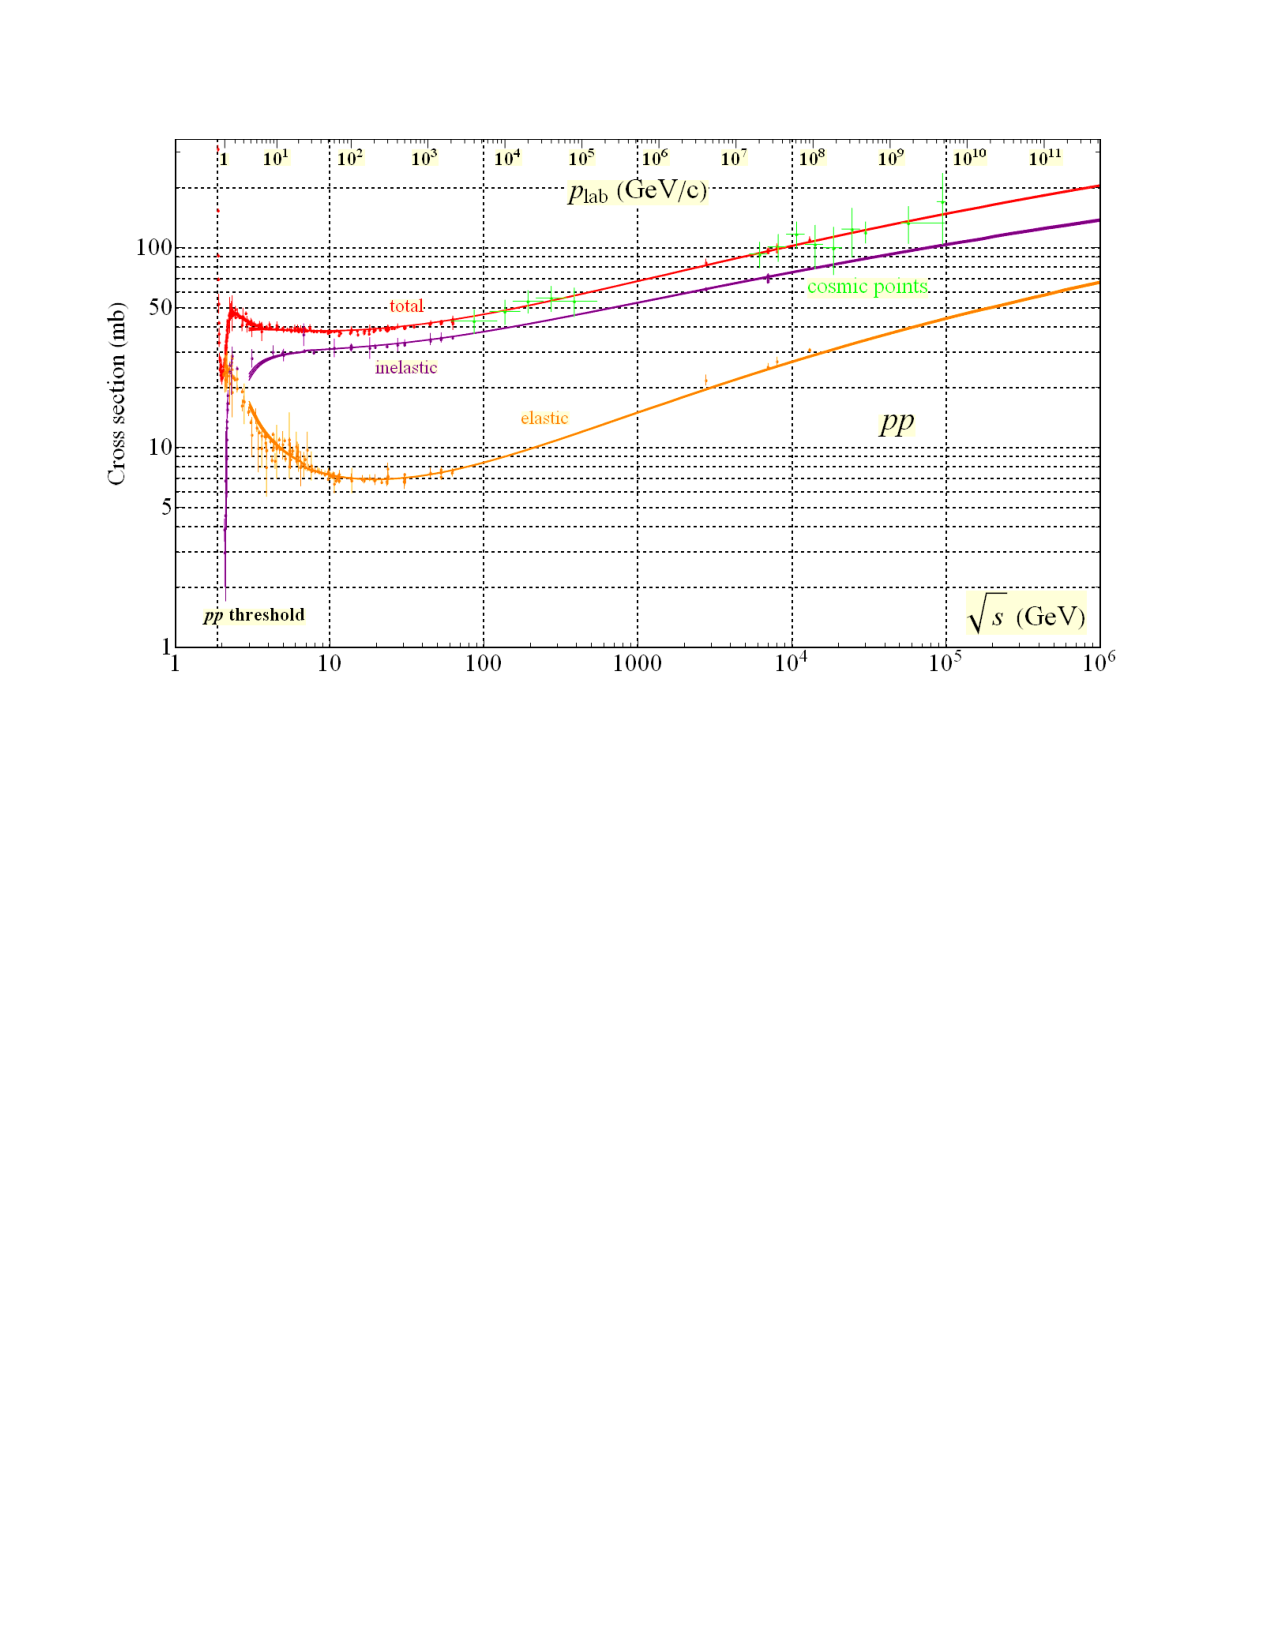
\includegraphics[width=0.6\textwidth]{chap2/pdg_pp_cross_section.pdf}
    \caption[Total, elastic, and inelastic $pp$ cross sections versus
             $p_{lab}$ and $\sqrt{s}$.]{
             Total, elastic, and inelastic $pp$ cross sections versus
             $p_{lab}$ and $\sqrt{s}$.
             Note that the total cross section is relatively constant over the
             range of momenta studied in E12-06-107, about
             \SIrange{4}{10}{\giga\electronvolt}.
             Figure reproduced from Ref~\cite{pdg_2020}.
            }
    \label{fig:pdg_pp_cross_section}
\end{figure}

% TODO: expand here
Use the PWIA approximation to measure transparency

\begin{equation}
    T(Q^2) = \frac{\int_V \, d^3p_m \, dE_m \, Y_{exp}(E_m, \vec{p}_m)}
                  {\int_V \, d^3p_m \, dE_m \, Y_{PWIA}(E_m, \vec{p}_m)}
\end{equation}

Previous transparency measurements, compiled in Fig~\ref{fig:aeep}, were taken
at SLAC, MIT Bates, and JLab for several nuclear targets.
These transparency measurements are independent of $Q^2$ over the range of 2 to
\SI{8}{\giga\electronvolt}.
This is consistent with the Glauber prediction, which is to say, an absence of
color transparency.
%TODO: Cite the models.

% TODO: Do we have a PDF version of this?
\begin{figure}[!h]
    \centering
    \includegraphics[width=0.6\textwidth]{chap2/aeep_transparency.png}
    \caption[Transparency measurements from several experiments studying
             quasielastic electron scattering from deuterium, carbon, iron,
             and gold.]{Transparency measurements from several experiments studying
             quasielastic electron scattering from deuterium, carbon, iron,
             and gold.
             Data taken at JLab~\cite{Abbot_1998, Garrow_2002, Rohe_2005} are shown as solid points.
             Data taken at SLAC~\cite{Makins_1994, ONeill_1995} are shown as large open symbols.
             Data taken at Bates~\cite{Garino_1992} are shown as small open symbols.
             The dotted line is a Glauber calculation from~\cite{Pandharipande_1992} for carbon data..
             Solid lines are constant-value fits to data above \SI{2}{\giga\electronvolt}.
            }
    \label{fig:aeep}
\end{figure}


\subsection{Pion photoproduction}
The onset of color transparency in pion photoproduction was studied at JLab,
using Bremsstrahlung photons generated by the CEBAF beam incident on a copper
radiator~\cite{Dutta_2003}.
Transparency was measured by taking the ratio of \ch{{^4}He} to \ch{{^2}H} cross sections at two
angles.
These measurements are shown in Fig~\ref{fig:pion_photoproduction_transparency}
along with two models.
The first model is a Glauber calculation, using exact ground state wave
functions~\cite{Arriaga_1995}.
The second adds CT to this model using the quantum diffusion model's modified hN
cross section~\cite{Farrar_1988}.

\begin{figure}[!h]
    \centering
    \includegraphics[width=0.6\textwidth]{chap2/pion_photoproduction_transparency.pdf}
    \caption[Nuclear transparency for $\ch{^{4}He}(\gamma,p\pi^+)$ at
            $\theta_{CM}=\ang{70}$ and $\theta_{CM}=\ang{90}$ as
            a function of 4-momentum transfer $\left|t\right|$.]{Nuclear transparency for $\ch{^{4}He}(\gamma,p\pi^+)$ at
            $\theta_{CM}=\ang{70}$ (left) and $\theta_{CM}=\ang{90}$ (right) as
            a function of 4-momentum transfer $\left|t\right|$.
            The inner bars are statistical uncertainties only.
            The outer bars are the statistical and point-to-point systematic
            uncertainties added in quadrature.
            The lower shaded band represents the prediction of a traditional
            Glauber calculation based on ground state wave functions for
            $\ch{^4He}$~\cite{Arriaga_1995}.
            The upper shaded band adds CT to this model using a modified
            hadron-nucleus cross section~\cite{Farrar_1988}.
            }
    \label{fig:pion_photoproduction_transparency}
\end{figure}

The slope of the measured transparencies' dependence on $Q^2$ is within one
$\sigma$ (two $\sigma$) of the Glauber calculation for the
$\theta_{CM}=\ang{70}(=\ang{90})$ data.
The data seem to deviate from the Glauber prediction, but a subsequent analysis
using a relativistic Glauber approximation showed that these
data are not conclusive evidence of the onset of CT \cite{Cosyn_2006}.


\subsection{Pion electroproduction}
The piCT experiment at JLab measured the $A$ and $Q^2$ dependence of the pion
cross section for several targets (\ch{^1H}, \ch{^2H}, \ch{^{12}C},
\ch{^{27}Al}, \ch{^{63}Cu}, and \ch{^{197}Au})~\cite{Clasie_2007, Qian_2010}.
Ref~\cite{Clasie_2007} defines nuclear transparency $T$ as the ratio of the pion
electroproduction cross section from a given nuclear target to the cross
section for a free proton, while Ref~\cite{Qian_2010} defines nuclear
transparency $T_D$ using the deuteron cross section in the denominator.
The purpose of this definition is to reduce uncertainty stemming from
the unknown pion electroproduction off a neutron and uncertainty in Fermi
smearing.
The deuterium nuclear transparency measurements are relatively independent of
$Q^2$, so both definitions show similar $Q^2$ dependencies in
Ref~\cite{Qian_2010}.
The transparency results are shown in
Fig~\ref{fig:pion_electroproduction_transparency_Q2_dependence} along with three
model predictions described below.

\begin{figure}[!h]
    \centering
    \includegraphics[width=0.6\textwidth]{chap2/pion_electroproduction_transparency_Q2_dependence.pdf}
    \caption{
            }
    \label{fig:pion_electroproduction_transparency_Q2_dependence}
\end{figure}

Larson et al.~\cite{Larson_2006} use a semiclassical formula based on the
eikonal approximation and a parameterization of final state interactions in
terms of an effective cross section based on a quantum diffusion
model~\cite{Farrar_1988}, in which the strength of the interaction is
proportional to the pion's propagation distance through the nucleus.
The transparency is given by a single integral over the path of the outgoing
pion, where the nuclear density $\rho(r)$ is of Woods-Saxon form,
\begin{equation}
    T = \frac{1}{A}\int d^3 \, r \rho(r)
           \exp{
                 -\int_z^\infty dz' \, \sigma_{eff} (z'-z,p_\pi) \rho(r')
               }
\end{equation}


Cosyn et al.~\cite{Cosyn_2008} calculate nuclear transparency as a ratio of
differential cross sections (integrated over the kinematic range of the
experiment) in a relativistic multiple scattering Glauber approximation (RMSGA)
to that in a relativistic plane wave impulse approximation (RPWIA).
All particles are taken to be plane waves in the RPWIA, while in the RMSGA
the wavefunctions of the outgoing pion and spectator nucleon are a convolution
of a plane wave with an eikonal phase operator that parameterizes the final
state interactions.
This model implements CT in this operator using the same quantum
diffusion model's effective cross section~\cite{Farrar_1988} used by Larson et
al.
This model also includes the effects of short range correlations, which create
local fluctuations in nuclear density.


Kaskulov et al.~\cite{Kaskulov_2009, Kaskulov_2012} calculate nuclear
transparency as a ratio of the differential cross sections from two variations
of the same model, one with and one without final state interactions.
This model is based on a microscopic description of pion
electroproduction from hydrogen~\cite{Kaskulov_2008}.
The nuclear reaction is broken up into hard partonic DIS and soft hadronic
components.
It is assumed that the beam electron interacts with a
nucleon in the nucleus the way it would with a free nucleon (also taking into
account Fermi motion, Pauli blocking, and nuclear shadowing).
The time development of the PLC is determined by the quantum diffusion
model~\cite{Farrar_1988}, with formation and production times determined by
Monte Carlo simulation of the Lund string hadronization
model~\cite{Anderson_1983} as described in Ref~\cite{Gallmeister_2005}.
The produced hadrons are then propagated through the nuclear medium using the
Boltzmann-Uehling-Uhlenbeck (BUU) equation.
This propagation models elastic and inelastic rescattering of outgoing hadrons.


The results of the piCT experiment are in agreement with the CT predictions of
Larson et al., while Cosyn et al. and Kaskulov et al. overestimate the $P_\pi$
and $Q^2$ dependence of the data.
Nevertheless, the observed increase in nuclear transparency is consistent with
CT.


In addition to studying the $Q^2$ dependence of nuclear transparency, piCT
fit the data to the form $T=A^{\alpha(Q^2)-1}$ where $A$ is the
number of nucleons in the nucleus and $\alpha(Q^2)$ is a free parameter.
The results of this fit along with the predictions of Larson et al. and Cosyn et
al. are shown in Fig~\ref{fig:pion_electroproduction_transparency_A_dependence}.
These results show a clear difference from the prediction of the Glauber model
without CT.

\begin{figure}[!h]
    \centering
    \includegraphics[width=0.6\textwidth]{chap2/pion_electroproduction_transparency_A_dependence.pdf}
    \caption[The parameter $\alpha(Q^2)$ extracted from the form
            $T=A^{\alpha(Q^2)-1}$
            fit to nuclear transparency measured by the piCT experiment.]{
            The parameter $\alpha(Q^2)$ extracted from the form
            $T=A^{\alpha(Q^2)-1}$
            fit to nuclear transparency measured by the piCT experiment.
            The inner bars are statistical uncertainties only.
            The outer bars are the statistical, systematic, and model
            uncertainties added in quadrature.
            Red points are data taken with low transverse photon polarization
            ($\epsilon\approx0.25$).
            Black points are data taken with high transverse photon polarization
            ($\epsilon\approx0.5$).
            The solid, dashed and dotted lines are the predictions of
            the Glauber model of Ref~\cite{Larson_2006},
            the Glauber+CT model of Ref~\cite{Larson_2006},
            and the Glauber+CT+SRC model of Ref~\cite{Cosyn_2006},
            respectively.
            }
    \label{fig:pion_electroproduction_transparency_A_dependence}
\end{figure}

\subsection{$\rho^0$ meson leptoproduction}
Because of the hadronic structure of high energy photons,
a virtual photon can fluctuate to a small $q\bar{q}$ state with mass $M_{qq}$
and propagate through a nucleus.
The formation length $l_{fr}=2\nu/(Q^2+M^2_{qq})$ refers to the distance over
which this $q\bar{q}$ state is frozen.
The coherence length $l_c=2\nu/(m^2_{v'}-m^2_{v})$ refers to the distance over
which the small $q\bar{q}$ state grows to a normal size $\rho^0$ meson,
where $m_v$ is the mass of the $\rho^0$ in its ground state
and $m_{v'}\approx\SI{1.5}{\giga\electronvolt}$ is the mass of the lowest $\rho$
excited state.


The results of early exclusive diffractive $\rho_0$ leptoproduction
experiments in the 1990s were suggestive of the onset of CT, but had limited
statistical power.
Another factor complicating the study of CT in this process is the
need to separate the effects of $l_{fr}$ and $l_c$.
If one is not careful, an increase in nuclear transparency with decreasing
$l_{fr}$ can be mistaken for an increase with $Q^2$, the signature of CT.


The first measurements of nuclear transparency for incoherent diffractive
$\rho^0$ leptoproduction were performed
at Fermilab by the E665 collaboration \cite{Adams_1995} and
at CERN by the NMC collaboration \cite{Arneodo_1994}
using muon beams of \SI{450}{\giga\electronvolt} and
\SI{200}{\giga\electronvolt} respectively.
At these energies, the $l_{fr}$ is comparable to the nuclear radius and
the $l_c$ is much larger than the nuclear radius; the $q\bar{q}$
state is frozen.

E665 took data with hydrogen, deuterium, carbon, calcium, and lead targets,
while NMC took data with deuterium,carbon and calcium targets.
The results for carbon and calcium, shown together in
Fig~\ref{fig:nmc_e665_transparency}, are consistent
with each other and show a slight increase in transparency.
This is only suggestive of an onset of CT due to limited statistics and
substantial background.

\begin{figure}[!h]
    \centering
    \includegraphics[width=0.7\textwidth]{chap2/nmc_e665_transparency.pdf}
    \caption[Transparency versus $Q^2$ for $\rho^0$ leptoproduction.]{Transparency versus $Q^2$ for $\rho^0$ leptoproduction.
             Filled symbols are data from NMC~\cite{Arneodo_1994}.
             Open symbols are data from E665~\cite{Adams_1995}.
            }
    \label{fig:nmc_e665_transparency}
\end{figure}


E665 also studied the $A$-dependence of the cross section, fitting their data
for all targets to a power law, $\sigma_A=\sigma_0A^\alpha(Q^2)$ where both
$\sigma_0$ and $\alpha$ are free parameters.
The extracted value of $\alpha$ at low $Q^2$ is consistent with soft nuclear
interactions.
The increase of $\alpha$ at higher $Q^2$ is again only suggestive of CT due to
the large uncertainty.


The HERMES collaboration at DESY~\cite{Ackerstaff_1999} measured nuclear
transparency as a function of $Q^2$ and $l_{fr}$ for coherent and incoherent
$\rho^0$ leptoproduction from \ch{^{14}N} using a \SI{27.5}{\giga\electronvolt}
positron beam.
Their measurements for exclusive incoherent electroproduction, shown in
Fig~\ref{fig:ackerstaff99}, show an increase in transparency at lower $l_{fr}$ consistent with an
introduction of initial state interactions between the nuclear medium and the
$q\bar{q}$ pair when the pair remains small for a distance smaller than
mean free path of a $\rho^0$ meson.

\begin{figure}[!h]
    \centering
    \includegraphics[width=0.5\textwidth]{chap2/ackerstaff99.pdf}
    \caption[Transparency versus coherence length for $\rho^0$ leptoproduction
             from hydrogen, helium, and nitrogen targets.]{Transparency versus coherence length for $\rho^0$ leptoproduction
             from hydrogen, helium, and nitrogen targets.
             These results demonstrate interactions of $q\bar{q}$ states with
             the nuclear medium at larger coherence lengths.
             Open circles are data from E665~\cite{Adams_1995} taken with muons.
             Open diamonds are data~\cite{McClellan_1969} taken with photons.
             Filled circles are data from HERMES~\cite{Ackerstaff_1999} taken
             with electrons.
             The error bars include statistical and point- to-point systematic
             uncertainties added in quadrature.
             The dashed line is the result of a Glauber model~\cite{Hufner_1996}.
            }
    \label{fig:ackerstaff99}
\end{figure}


Because $l_{fr}$ is comparable the nuclear radius in this experiment, these
measurements depend on $l_c$.
As such, the collaboration studied the nuclear transparency's $Q^2$-dependence
while keeping $l_{fr}$ fixed~\cite{Airapetian_2003}.
Transparencies for coherent and incoherent $rho^0$ electroproduction were
extracted for fixed $(l_{fr},Q^2)$ bins, as shown in
Fig~\ref{fig:airapetian_T_vs_lfr}.
Due to low statistics, the transparencies were fit to a form
$P_0 + P_1 \cdot Q^2$, where $P_0$ is a free parameter for each $l_fr$ bin and
the slope $P_1$ is a common free parameter among the bins.

\begin{figure}[!h]
    \centering
    \begin{subfigure}[b]{0.475\textwidth}
        \centering
        \includegraphics[width=\textwidth]{chap2/airapetian_coherent.pdf}
        \caption{Coherent $\rho^0$ production.}
        \label{fig:airapetian_coherent}
    \end{subfigure}
    % \hfill
    \begin{subfigure}[b]{0.475\textwidth}
        \centering
        \includegraphics[width=\textwidth]{chap2/airapetian_incoherent.pdf}
        \caption{Coherent $\rho^0$ production.}
        \label{fig:airapetian_incoherent}
    \end{subfigure}
    \caption[Transparency versus $Q^2$ for varying bins of coherence length.]{
             Transparency versus $Q^2$ for bins of coherence length
             indicated by a label at the top right of each panel.
             The straight line is the result of the fit to the $Q^2$-dependence
             of all bins.
             Error bars represent statistical uncertainties.
            }
    \label{fig:airapetian_T_vs_lfr}
\end{figure}

The extracted slopes for incoherent and coherent production were $0.70\pm0.21$
and \SI{0.089\pm0.046}{\per\giga\electronvolt\squared} respectively.
These slopes agree with the predictions of a model using the light cone Green
function formalism, incorporating the effects of coherence length and
CT~\cite{Kopeliovich_2002}.
As with the E665 and NMC results, the HERMES results are only suggestive of the
onset of CT due to their limited statistics.


The CLAS collaboration measured nuclear transparency for exclusive
incoherent $\rho^0$ production off carbon and iron relative to deuterium using
a \SI{5}{\giga\electronvolt} electron beam at JLab~\cite{ElFassi_2012}.
% The $t$ distributions were fit to a form $Ae^{-bt}$.
As seen in Fig~\ref{fig:clas_T_vs_lfr}, these transparencies are independent of
$l_{fr}$ because $l_{fr}$ (\SIrange{\sim0.5}{0.9}{\femto\meter}) is smaller
than the nuclear radii of carbon and iron, \SI{2.9}{\femto\meter} and
\SI{4.6}{\femto\meter} respectively.
As a result, any increase in transparency as a function of $Q^2$ cannot be a
result of varying $l_{fr}$, but rather a signal of CT.

\begin{figure}[!h]
    \centering
    \includegraphics[width=0.7\textwidth]{chap2/clas_T_vs_lfr.pdf}
    \caption[Nuclear transparency as a function of $l_{fr}$.]{
            Nuclear transparency as a function of $l_{fr}$.
            The inner error bars are statistical uncertainties.
            The outer error bars are the quadrature sum of statistical and
            systematic uncertainties.
            The carbon data has been scaled by a constant to fit in the same
            figure with the iron data.
            }
    \label{fig:clas_T_vs_lfr}
\end{figure}

The $Q^2$ dependence of these transparency measurements is shown in
Fig~\ref{fig:clas_T_vs_Q2} along with the predictions of two models.
The Frankfurt-Miller-Strikman (FMS) model~\cite{Frankfurt_2008} uses a standard
Glauber calculation, using the quantum diffusion model's modified
hadron-nucleus cross section~\cite{Farrar_1988} to implement CT. This model
also includes the effects of the decay of the $\rho^0$ meson.
The Gallmestier-Kaskulov-Mosel (GKM) model~\cite{Gallmeister_2011} is similar
to Kaskulov et al.'s model~\cite{Kaskulov_2008} of pion electroproduction,
which uses the BUU formalism to transport (pre)hadrons through the nucleus.
Both models predict the behavior of the CLAS carbon data quite well, but the
GKM modek underestimates the iron transparency.

\begin{figure}[!h]
    \centering
    \includegraphics[width=0.7\textwidth]{chap2/clas_T_vs_Q2.pdf}
    \caption[Nuclear transparency as a function of $Q^2$.]{
            Nuclear transparency as a function of $Q^2$.
            The inner error bars are statistical uncertainties.
            The outer error bars are the quadrature sum of statistical and
            systematic uncertainties.
            The curves are predictions of the
            FMS~\cite{Frankfurt_2008} (red)
            and
            GKM~\cite{Gallmeister_2011} (green)
            models with (dashed–dotted and dashed curves, respectively)
            and
            without (dotted and solid curves, respectively)
            the effetcs of CT.
            Both models include the pion absorption effect when the $\rho^0$
            meson decays inside the nucleus.
            }
    \label{fig:clas_T_vs_Q2}
\end{figure}


These data were also fit to a linear form $T=aQ^2+b$,
and the slope $a$ was compared to the predictions of the above two models as
well as a third, the Kopeliovich-Nemchick-Schmidt (KNS)
model~\cite{Kopeliovich_2007}.
The KNS model uses the same light cone Green function formalism used in the
context of the HERMES $\rho^0$ production data.
The results of these fits and the model predictions are shown in
Table~\ref{tab:CLAS_slopes}.

\begin{table}[h]
    \centering
    \caption[Slope parameters from a fit to the $Q^2$ dependence of CLAS
            nuclear transparency data taken for carbon and
            iron]{
            Slope parameters from a fit to the $Q^2$ dependence of CLAS
            nuclear transparency data taken for carbon and
            iron~\cite{ElFassi_2012}. Also shown are predictions of the
            KNS~\cite{Kopeliovich_2007},
            GKM~\cite{Gallmeister_2011}, and
            FMS~\cite{Frankfurt_2008} models.
            }
    \begin{tabular}{ccccc}
\specialrule{.1em}{.05em}{.05em}
         Nucleus &  Measured slopes (\si{\per\giga\electronvolt\squared}) & \multicolumn{3}{c}{Model predictions} \\ \cline{3-5}
                 &                                                        &  KNS  &  GKM  &  FMS                  \\
\specialrule{.1em}{.05em}{.05em}
         C       &  $0.044\pm0.015_{stat}\pm0.019_{sys}$                  & 0.06  & 0.06  & 0.025                 \\
         Fe      &  $0.053\pm0.008_{stat}\pm0.013_{sys}$                  & 0.047 & 0.047 & 0.032                 \\
\specialrule{.1em}{.05em}{.05em}
    \end{tabular}
    \label{tab:CLAS_slopes}
\end{table}


\section{Summary}
Taken together, these experiments show support for the existence of CT, as well
as observation of its onset for scattering processes involving mesons.
Such evidence for processes involving hadrons has not yet been demonstrated.
This may be because the onset for a $qqq$ PLC will necessarily be higher in
$Q^2$ than that of a $q\bar{q}$ pair.

Other reviews of theoretical considerations and previous experiments can be found in
the recent articles by Dutta, Hafidi, and Strikman~\cite{Dutta_2013,Dutta_2012}.

\include{chap3}
\include{chap4}
\chapter{Results}
\section{Missing Energy and Missing Momentum}

Figures~\ref{fig:Report_h8.pdf_pg3} through~\ref{fig:Report_c143_sm.pdf_pg3}
compare distributions of physics quantities measured in experiment (in blue)
and from simulation (in red).
These figures' panels show missing energy invariant mass $W$, missing energy,
missing momentum, and $p_{mz}$, the component of missing momentum parallel to
the 3-momentum transfer $\vec{q}$.
The shapes of the missing energy spectra for $H(e,e'p)$ data disagree in the
region between 0 and $\sim\SI{50}{\mega\electronvolt}$
because SIMC does not include any smearing of reconstructed momenta that
results from the spectrometers' finite resolution.
To obtain our transparency measurements for $H(e,e'p)$ we integrate these
distributions over $E_{m}<\SI{100}{\mega\electronvolt}$, so this distortion
does not affect out results.

The tail of the missing momentum distributions above
$\SI{300}{\mega\electronvolt}$ is lower in simulation than experiment.
This is likely because short range correlations~\cite{Fomin_2017}
drive nucleons to higher missing momenta than is accounted for by the
spectral functions used in SIMC.
% In addition, the simulated $p_m$ distributions only include quasielastic
% scattering.
% The experimental distributions are not drawn with a cut on $E_{m}$,
% so may include some contributions from pion electroproduction.
For ${}^{12}C(e,e'p)$ we integrate the yield over the
$\vec{p}<\SI{300}{\mega\electronvolt}$ region so
our transparency measurements are insensitive to the
divergence above this limit.


Similar comparisons of target variables are contained in
Appendix~\label{app:distributions}.


\begin{figure}[!h]
    \centering
    \includegraphics[page=3,width=1.0\textwidth]{pass5_report/Report_h8.pdf}
    \caption{
            Experimental (in blue) and Monte Carlo (in red) distributions of
            reconstructed physics quantities for
            the $LH_2$ target at $Q^2=\SI{8.0}{\giga\electronvolt\squared}$.
            }
    \label{fig:Report_h8.pdf_pg3}
\end{figure}


\begin{figure}[!h]
    \centering
    \includegraphics[page=3,width=1.0\textwidth]{pass5_report/Report_h95sm.pdf}
    \caption{
            Experimental (in blue) and Monte Carlo (in red) distributions of
            reconstructed physics quantities for
            the $LH_2$ target at $Q^2=\SI{9.5}{\giga\electronvolt\squared}$.
            }
    \label{fig:Report_h95sm.pdf_pg3}
\end{figure}


\begin{figure}[!h]
    \centering
    \includegraphics[page=3,width=1.0\textwidth]{pass5_report/Report_h115.pdf}
    \caption{
            Experimental (in blue) and Monte Carlo (in red) distributions of
            reconstructed physics quantities for
            the $LH_2$ target at $Q^2=\SI{11.5}{\giga\electronvolt\squared}$.
            }
    \label{fig:Report_h115.pdf_pg3}
\end{figure}


\begin{figure}[!h]
    \centering
    \includegraphics[page=3,width=1.0\textwidth]{pass5_report/Report_h143.pdf}
    \caption{
            Experimental (in blue) and Monte Carlo (in red) distributions of
            reconstructed physics quantities for
            the $LH_2$ target at $Q^2=\SI{14.2}{\giga\electronvolt\squared}$.
            }
    \label{fig:Report_h143.pdf_pg3}
\end{figure}


\begin{figure}[!h]
    \centering
    \includegraphics[page=3,width=1.0\textwidth]{pass5_report/Report_c12_8.pdf}
    \caption{
            Experimental (in blue) and Monte Carlo (in red) distributions of
            reconstructed physics quantities for
            the ${}^{12}C$ target at $Q^2=\SI{8.0}{\giga\electronvolt\squared}$.
            }
    \label{fig:Report_c12_8.pdf_pg3}
\end{figure}


\begin{figure}[!h]
    \centering
    \includegraphics[page=3,width=1.0\textwidth]{pass5_report/Report_c95.pdf}
    \caption{
            Experimental (in blue) and Monte Carlo (in red) distributions of
            reconstructed physics quantities for
            the ${}^{12}C$ target at $Q^2=\SI{9.5}{\giga\electronvolt\squared}$.
            }
    \label{fig:Report_c95.pdf_pg3}
\end{figure}


\begin{figure}[!h]
    \centering
    \includegraphics[page=3,width=1.0\textwidth]{pass5_report/Report_c115.pdf}
    \caption{
            Experimental (in blue) and Monte Carlo (in red) distributions of
            reconstructed physics quantities for
            the ${}^{12}C$ target at $Q^2=\SI{11.5}{\giga\electronvolt\squared}$.
            }
    \label{fig:Report_c115.pdf_pg3}
\end{figure}


\begin{figure}[!h]
    \centering
    \includegraphics[page=3,width=1.0\textwidth]{pass5_report/Report_c143_sm.pdf}
    \caption{
            Experimental (in blue) and Monte Carlo (in red) distributions of
            reconstructed physics quantities for
            the ${}^{12}C$ target at $Q^2=\SI{14.2}{\giga\electronvolt\squared}$.
            }
    \label{fig:Report_c143_sm.pdf_pg3}
\end{figure}


\section{Nuclear Transparency}

The nuclear transparency was extracted as the ratio of the experimental yield
to the simulated PWIA yield from \textit{SIMC} over the phase space volume $V$
defined by the limits
$E_m<\SI{80}{\mega\electronvolt}$ and
$|\vec{p}_{miss}|<\SI{300}{\mega\electronvolt}$ for ${}^{12}C(e,e'p)$
and
$E_m<\SI{100}{\mega\electronvolt}$ and
$|\vec{p}_{miss}|<\SI{100}{\mega\electronvolt}$ for $H(e,e'p)$.
\begin{equation}
    T(Q^2) = \frac{\int_{V} d^{3} p_{m} d E_{m} Y_{exp }(E_{m}, \vec{p}_{m})}
                  {\int_{V} d^{3} p_{m} d E_{m} Y_{PWIA}(E_{m}, \vec{p}_{m})}
\end{equation}

The nuclear transparency measured as a function of $Q^2$ for $H(e,e'p)$ is
shown in Fig~\ref{fig:lh2_transparency_results}.
This elastic scattering process has no final state interactions and should be
accurately modeled by the PWIA as implemented in \textit{SIMC}.
The ratio $T$ should thus be equal to one for each point, and these
measurements are consistent with $T=1$ well within the statistical and
systematic uncertainty.
This indicates that the Monte Carlo simulation in \textit{SIMC} accurately
models the scattering process and that both the spectrometers and
\textit{hcana} are accurately reconstructing physics quantities.

% TODO: replace this with a pdf
\begin{figure}[!h]
    \centering
    \includegraphics[width=0.8\textwidth]{chap5/lh2_results.png}
    \caption[Nuclear transparency for $H(e,e'p)$ as a function of
            momentum transfer.]{
            Nuclear transparency for $H(e,e'p)$ as a function of
            momentum transfer.
            The error bars represent statistical uncertainty and the
            shaded band represents the 4.0\% systematic uncertainty.
            }
    \label{fig:lh2_transparency_results}
\end{figure}

The nuclear transparency measured as a function of $Q^2$ for ${}^{12}C(e,e'p)$
is shown in Fig~\ref{fig:lh2_transparency_results} along with previous
measurements.
Our measurements from 8--\SI{14.2}{\giga\electronvolt\squared} are consistent
with conventional multiple scattering calculations~\cite{Pandharipande_1992}
and do not support the onset of color transparency.

\begin{figure}[!h]
    \centering
    \includegraphics[width=0.8\textwidth]{chap5/c12_results.pdf}
    \caption[Nuclear transparency for ${}^{12}C(e,e'p)$ as a function of momentum transfer.]{
            Nuclear transparency for ${}^{12}C(e,e'p)$ as a function of
            momentum transfer.
            The results of this experiment, E12-06-107, are shown in red along
            with previous measurements in open shapes.
            The error bars represent statistical uncertainty and the
            shaded band represents the 4.0\% systematic uncertainty.
            The magenta line is the prediction of a Glauber
            model that does not include CT~\cite{Pandharipande_1992}.
            The dashed lines represent predictions, for two choices of
            parameters, of a model including CT~\cite{Frankfurt_1995_PRC}.
            The solid line represents the prediction of a relativistic Glauber
            model that includes CT~\cite{Cosyn_2006}.
            }
    \label{fig:c12_transparency_results}
\end{figure}

\subsection{Systematic Uncertainty}

Table~\ref{tab:systematic_uncertainty} lists the major sources of systematic
uncertainty in our measurements of nuclear transparency.


The systematic uncertainty due to spectrometer acceptance was estimated by
taking the average of the bin-wise difference between the normalized missing
momentum spectra for data and simulation.


The uncertainty due to event selection was estimated by varying the limits of
the cuts listed in Tables~\ref{tab:lh2_cuts} and~\ref{tab:c12_cuts}
by $\pm10\%$ one at a time
and calculating the corresponding percentage change in measured transparency.
The quadrature sum of these variations was used as the systematic uncertainty.


Tracking efficiency.


Radiative corrections.


The uncertainty due to livetime and the detector efficiencies was determined
from a set of luminosity scans taken with the ${}^{12}C$ target.
The charge-normalized yield from these scans for each spectrometer was found to
be independent of the beam current within statistical uncertainties,
The average variation in the normalized yield vs beam current was recorded as the
systematic uncertainty (0.5\%).


The normalization uncertainty due to the free $ep$ cross section used in
\textit{SIMC} is 1.8\%~\cite{Bosted_1995}.
The uncertainty due to target thickness is taken from the JLab target group's
measurements. %TODO: find this citation again
The uncertainty in measured charge was estimated to be $1\%$ by varying the
minimum beam current cut used by \textit{hcana} to calculate each run's average
current.
Proton absorption.

% The total model-dependent uncertainty is 3.9\% when the uncertainty in the
% spectral function (2.8\%) and the corrections due to nucleon-nucleon
% correlations (2.7\%) are added in quadrature.

% The uncertainty in the spectral function includes the effects of the off-shell
% $\sigma_{ep}$ of 2\%, the electric and magnetic form factors of the proton
% (2\%) as previously determined\,\cite{ONeill_1995}.

\begin{table}[htb!]
    \caption[Systematic uncertainties in our measurements of nuclear
        transparency.]{
        Systematic uncertainties in our measurements of nuclear
        transparency.
        $Q^2$-dependent uncertainties are averaged over all kinematic settings.
        The total uncertainty is the quadrature sum of the individual
        contributions.
    }
    \label{tab:systematic_uncertainty}
    \centering
    \begin{tabular}{lc}
\specialrule{.1em}{.05em}{.05em}
        Source                            & $Q^2$-dependent uncertainty (\%) \\
\specialrule{.1em}{.05em}{.05em}
        Spectrometer acceptance           & 2.6                              \\
        Event selection                   & 1.4                              \\
        Tracking efficiency               & 0.5                              \\
        Radiative corrections             & 1.0                              \\
        Live time \& detector efficiency  & 0.5                              \\
\specialrule{.1em}{.05em}{.05em}
        Source                            & Normalization uncertainty (\%)   \\
\specialrule{.1em}{.05em}{.05em}
        Free $ep$ cross section           & 1.8                              \\
        Target thickness                  & 0.5                              \\
        Beam charge                       & 1.0                              \\
        Proton absorption                 & 1.2                              \\
\specialrule{.1em}{.05em}{.05em}
        Total                             & 4.0                              \\
\specialrule{.1em}{.05em}{.05em}
    \end{tabular}
\end{table}


\chapter{Summary and Conclusion}
Using the upgraded 12\,\,GeV CEBAF beam at JLab, coincidence $(e,e'p)$ data
were taken with $^{1}H$ and $^{12}C$ targets for $Q^2$ values between 8 and
14.2\,(GeV/$c)^2$.
Nuclear transparencies were extracted for each kinematic point by integrating
charge-normalized yields and taking their ratio.
The transparency measured at the lowest kinematic point at
$Q^2=8.1$\,(GeV/$c)^2$ agrees with prior measurements at JLab.
The $Q^2$-dependence of the measured transparencies is consistent with
traditional Glauber multiple scattering theory and does not show an onset of
color transparency in $^{12}C(e,e'p)$ below $Q^2=14.2$\,(GeV/$c)^2$.
% Though other work has suggested that the onset may be more obvious in the
% $s$-shell than in the $p$-shell, this effect is not evident in this
% experiment's results.

As discussed in Sec~\ref{sec:ct_def}, Brodsky and de Téramond~\cite{Brodsky_2021}
use light-front holographic QCD to derive an expression for a PLCs transverse
size as a function of twist $\tau$ and $Q^2$.
Their calculations suggest that the onset of CT in ${}^{12}C(e,e'p)$ may be
higher than what can currently be probed in Hall C, perhaps not occurring
until $Q^2=\SI{20}{\giga\electronvolt\squared}$.

Using the same framework, Caplow-Munro and Miller~\cite{CaplowMunro_2021}
demonstrate that expansion effects are not sufficiently large to cause FSI in
this experiment's measurements.
The lack of a rise in transparency then suggests that a PLC was not formed,
and that the proton's electromagnetic form factor is dominated at large
momentum by the Feynman mechanism\footnote{In the Feynman mechanism, a single
quark carrying a large portion of a hadron's momentum absorbs the entire
momentum transfer $Q$~\cite{Drell_1970}.} rather than a PLC.

Experiments at JLab in the near future will include color transparency studies in $\rho$ (Hall B) and $\pi$ (Hall C) electroproduction, and $\pi$ photoproduction in Hall D.

\appendix
\include{appendices}

\newpage
\cleardoublepage

\cleardoublepage
\pdfbookmark[0]{Bibliography}{Bibliography}
\include{biblio}
\cleardoublepage

\end{document}
